% !TEX encoding = UTF-8 Unicode
\documentclass[fleqn,twoside]{article}
\usepackage[ngerman]{babel}
\usepackage[utf8]{inputenc}
\usepackage[T1]{fontenc}
\usepackage{graphicx}
\usepackage{fancyhdr}
\usepackage{amssymb}
\usepackage{amsmath}
\usepackage{cite}
\usepackage{eurosym}
\usepackage{wrapfig}
\usepackage{tabularx}
\usepackage{pdfpages}
\usepackage{nicefrac}
\usepackage{wasysym}
\usepackage{multirow}
\usepackage{pifont}
\usepackage{textcomp}
\usepackage{comment}
\usepackage{units}
%\usepackage{siunitx}
\usepackage{yfonts}
\usepackage{calligra}
\usepackage{csquotes}
%\usepackage{emerald}
\usepackage{titlesec}
\usepackage{tikz}
\usepackage{stanli}
\usepackage{romanbar}
\usepackage{graphicx}
\usepackage{tabto}
\usepackage{todonotes}
%\usepackage{3dstructuralanalysis}
%\usepackage{structuralanalysis}
\usepackage{enumitem}
\usepackage{booktabs}
\usepackage{float}


%Befehle abändern
%Itemize ohne Lücken
\setlist[itemize]{noitemsep, parsep=0pt, topsep=2pt}
\raggedbottom
%\renewcommand{\todo}[1]{\todo[inline]{#1}}


%Betragsfunktion
\newcommand{\abs}[1]{\ensuremath{\left\vert#1\right\vert}}
%Einheitenfunktion
\newcommand{\un}[2]{{\unit[#1]{\color{black!80}[#2]}}}

\usepackage[pdftex, colorlinks, linkcolor=black, frenchlinks]{hyperref}
\usepackage[a4paper , lmargin = {2.5cm} , rmargin = {2cm} , tmargin = {2.5cm} , bmargin = {2.5cm} ]{geometry}
\pagestyle{fancy}

\title{\Huge{\textfrak{Felsmechanik und Tunnelbau \\Formelsammlung}}}
\author{\calligra{Jonathan C. Walter}\\\calligra{Jonas H. Konrad}}
\date{\textfrak{\today}}

\begin{document}
\parindent 0pt
\fancyhead[L]{Jonathan C. Walter, Jonas H. Konrad}
\fancyfoot[L]{\frakfamily J. C. W.;J. H. K.}
\fancyfoot[R]{\frakfamily }
\fancyfoot[C]{\frakfamily Vor der Hacke ist es duster. \\Seite \thepage}
\maketitle \thispagestyle{empty}
%\initfamily %Für Initialien
\begin{center}
\textfrak{Diese Formelsammlung wurde im Sommersemester 2022 von Jonathan Walter und Jonas Konrad verfasst.\\Kein Anspruch auf Vollständigkeit oder Fehlerfreiheit.\\LaTex Vorlage:github.com/Neowise33}
\end{center}
\tableofcontents
%\listoftodos
%\newpage

\section{Theoriewissen}

\begin{itemize}
\item Mineralogische Abkürzungen:\\
    \begin{tabular}[t]{p{1cm}p{3cm}}
         Q & = Quarz\\
         Fsp & = Feldspat\\
         Amph & = Amphibol\\
         Px & = Pyroxen
    \end{tabular}
\item Größenordnung Gebirgswichte: $2,65 < \varrho < 2,75 \left[ \frac{g}{cm^3} \right]$
\item Trennflächen und deren Raumstellung: Notation:\\KK:(Winkel in Ebene($0^\circ$ nach rechts)/(Winkel im Schnitt($0^\circ$ in Ebene))
\end{itemize}

\section{Allgemeine Annahmen/Gesetzmäßigkeiten}

\begin{itemize}
        %\item Spannungszustand:
        %$\left\{\begin{array}{ll}
                %\text{Primär}: & \sigma_v \& \sigma_h  \\
                %\text{Sekundär:} & \sigma_r=0 \& \sigma_\theta=2\sigma_v
            %\end{array}\right.$
    \item Seitendruckbeiwert: $\lambda = K_0 = 1-\sin\varphi$ ; ($\varphi=30^\circ \Rightarrow K_0 = 0,5$)
    %\item Mohr-Coulomb'sches Festigkeitskriterium: $\sigma_1 = \frac{1-\sin\varphi}{1+\sin\varphi}\sigma_3 - \frac{2c\cos\varphi}{1+\sin\varphi}$
    \item Bei großen Überlagerungen ist die Kohäsion vernachlässigbar: $\sigma_h > \frac{1-\sin\varphi}{1+\sin\varphi}\sigma_v = k_h \sigma_v$ ; $\lambda > \frac{1-\sin\varphi}{1+\sin\varphi}$
    \item Hook'sche Gleichung: $\lambda = \frac{\nu}{1-\nu}$ ($0<\nu<0,5$) ($\nu =\frac{\text{Radiale Dehnung}}{\text{Axiale Dehnung}}$)
    \item Seitendruckbeiwert Wasser: $\lambda=1$ 
\end{itemize}

\section{Felsmechanik}

\subsection{Spannungszustände}
\begin{itemize}
    \item Primär: $\sigma_v$; $\sigma_h$
    \item Sekundär: $\sigma_r=0$;  $\sigma_\theta=2\sigma_v$
\end{itemize}
%\section{Allgemeine Formel und Zusammenhänge}
\subsection{Versuche}

\subsubsection{Dreiaxialer Druckversuch}

\begin{itemize}
    \item MST-Grenzspannungsauswertung: $\sigma_1-\sigma_3=(\sigma_1+\sigma_3)\sin(\varphi)+2c_g\cdot\cos{\varphi}$ (Intakter Fels)
    \begin{itemize}
        \item Verformungsmodul: $\un{V}{MPa}=\frac{\Delta\sigma}{\Delta\epsilon}\cdot 100$ bei Erstbelastung
        \item Verformungsmodul: $\un{E}{MPa}=\frac{\Delta\sigma}{\Delta\epsilon_e}\cdot 100$ bei Wiederbelastung
    \end{itemize}
    \item $\sigma_1 = \sigma_v = \gamma z$ und $\sigma_3 = \sigma_h \lambda \sigma_v$ einsetzen und nach z auflösen $\Rightarrow$ Tiefe ab der Fels geklüftet vorliegt.
    \begin{itemize}
        \item $q=\frac{\sigma_1-\sigma_2}{2}$
        \item $p=\frac{\sigma_1+\sigma_2}{2}$
        \item $\varphi'=\arcsin(\tan(\alpha))$
        \begin{itemize}
            \item $\tan(\alpha)=\frac{\Delta q}{\Delta p}$
        \end{itemize}
        \item $c_g=\frac{b}{\cos(\varphi)}$
        \begin{itemize}
            \item $b=q-p\tan(\alpha)$
        \end{itemize}
    \end{itemize}
    \item Festigkeitsansatz nach John: $\sigma_1=\dfrac{\sigma_3\left[\sin(2\alpha_k-\varphi_k)+\sin(\varphi_k)\right]+2c_k\cos(\varphi_k)}{\sin(2\alpha_k-\varphi_k)-\sin(\varphi_k)}$ (geklüfteter Fels)
    \begin{itemize}
    \item $\tau=\sigma\tan(\varphi_k)+c_k=\frac{\sigma_1-\sigma_3}{2}\sin(2\alpha)$ (bilineares Kriterium)
    \item $\sigma=\frac{\sigma_1+\sigma_3}{2}+\frac{\sigma_1-\sigma_3}{2}\cos(2\alpha)$
    \begin{itemize}
        \item $\alpha$ = Kluftwinkel
        \item Schräge Spannungsmessungen mit $\omega$: $\alpha = \alpha_{Kluft} + \omega$ $_{\text{(März 2018 - 1)}}$
    \end{itemize}
    \end{itemize}
    \item Festigkeitsansatz nach Mohr-Coulomb: $\sigma_1=\frac{1+\sin(\varphi)}{1-\sin(\varphi)}\sigma_3+\frac{2c\cdot\cos(\varphi)}{1-\sin(\varphi)}$
    \begin{itemize}
        \item Im Tunnel: $\sigma_1=\sigma_{\theta}$ und $\sigma_3=\sigma_r$
    \end{itemize}
\end{itemize}

\subsubsection{Scherversuch}

\begin{itemize}
    \item $T=N\tan(\varphi) +c$
    \item Patton ($i$: Aufgleitwinkel) $\frac{S^*}{N^*}=\tan(\varphi)$
    \begin{itemize}
        \item $S^*=S\cos(i)-N\sin(i)$
        \item $N^*=N\cos(i)+S\sin(i)$
    \end{itemize}
    \item Ergebnisse: Restreibungswinkel: $\varphi$ ; Scherweg ; Dilatation
    \item $i=\arctan\left( \frac{\textit{Dilatation}}{\textit{Scherweg}}\right)$
    \item Haltende Spannung: $\sigma = \sigma_{n} \tan(\varphi + i)$ ; $\sigma_n = \sigma_\theta$
    \item Treibende Kraft: $\tau_{r \theta}$ nach Kirsch

\end{itemize}


\subsubsection{Spaltzugversuch (Tension-Cutoff Verfahren)}\label{Spaltzugversuch}

\begin{itemize}
    \item $\sigma_t=\dfrac{2F_B}{\pi dl}$
\end{itemize}

\subsubsection{Punktlastversuch}\label{Punktlastversuch}

\begin{itemize}
    \item $\sigma_c=\frac{F_c}{A}$
\end{itemize}

\subsubsection{Sondierungsversuch}
\begin{itemize}
    \item Horizontalspannung: $\sigma_h = \dfrac{P_i - \sigma_t}{2}$\\
    $\sigma_t =$ Zugfestigkeit; $P_i =$ maximaler Druck Sondierung
\end{itemize}

\subsection{Gebirgsklassifikation}
\subsubsection{RQD - Rock Quality Designation}
\begin{itemize}
    \item $RQD = \dfrac{100 \sum x_i}{L}$\\ 
    $x_i =$ Länge der Kernstücke in einem Kernabschnitt der Länge L, die länger als 10cm sind.
    \item Felsqualität:\\
        \begin{tabular}{|c|c|c|}
            \hline
            \textbf{RQD-Index} & \textbf{Felsqualität} & \textbf{Rock Quality} \\ \hline
            0-25               & sehr gering           & very poor             \\ \hline
            25-50              & gering                & poor                  \\ \hline
            50-75              & mittel                & fair                  \\ \hline
            75-90              & gut                   & good                  \\ \hline
            90-100             & ausgezeichnet         & excellent             \\ \hline
        \end{tabular}
\end{itemize}


\subsubsection{RMR - Rock Mass Rating}
\begin{itemize}
    \item $RMR = I_1 + I_2 + I_3 + I_4 + I_5 + I_6$
    \item 
    \begin{tabular}{l l l}
            $I_1$ = Gesteinsfestigkeit & $I_2$ = RQD-Index (Durchtrennungsgrad) & $I_3$ = Trennflächenabstand\\ 
            $I_4$ = Trennflächenzustand & $I_5$ = Bergwasserverhältnisse & $I_6$ = Trennflächenorientierung
    \end{tabular}
\end{itemize}
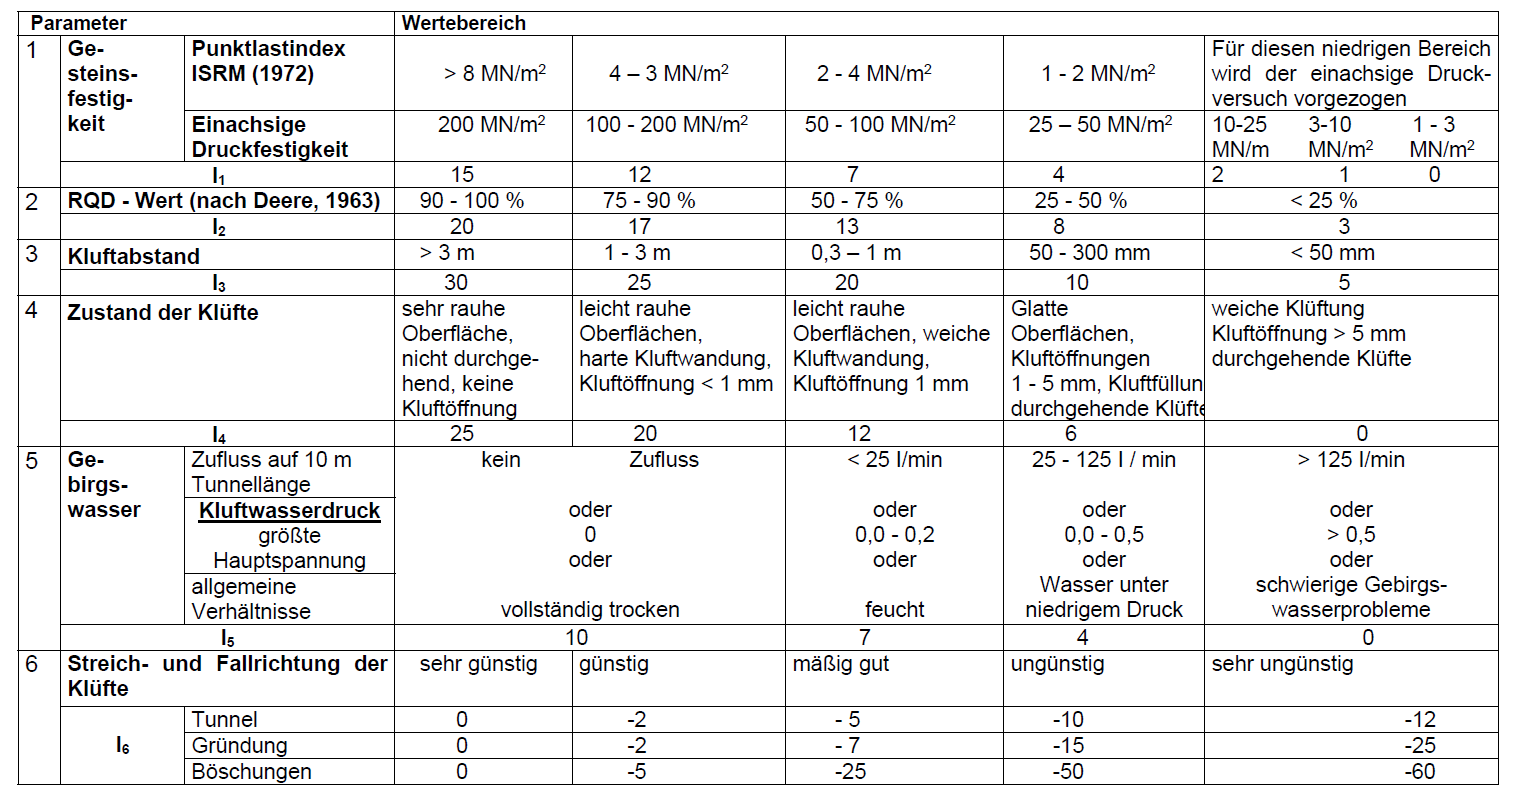
\includegraphics[width=1\textwidth]{Grafiken/RMR_Tabelle.png}

\subsubsection{Q-System}\label{Q}

\begin{itemize}
    \item $Q=\dfrac{RQD\cdot J_r\cdot J_w}{J_n\cdot J_a\cdot SRF}$
\end{itemize}
\begin{minipage}{0.5\textwidth}
    \begin{tabular}{|c|l|c|}\hline
            \multicolumn{2}{|c|}{Merkmale} & $J_n$ \\\hline
            A   & massiv, keine oder wenig Klüfte   & 0,5-1 \\
            B   & eine Kluftschar                   & 2     \\
            C   & eine Kuftschar mit Nebenkluft     & 3     \\
            D   & zwei Kuftschare                   & 4     \\
            E   & zwei Kuftschare mit Nebenkluft    & 6     \\
            F   & drei Kluftschare                  & 9     \\
            G   & drei Kluftschare mit Nebenkluft   & 12    \\
            H   & vier oder mehr Kluftschare        & 15    \\
            I   & zerrüttetes Gebirge (wie Erde)    & 20    \\\hline
            \multicolumn{3}{|l|}{-für Kreuzungen gilt $3J_n$}\\
            \multicolumn{3}{|l|}{-für Portale gilt $2J_n$}\\\hline
    \end{tabular}
    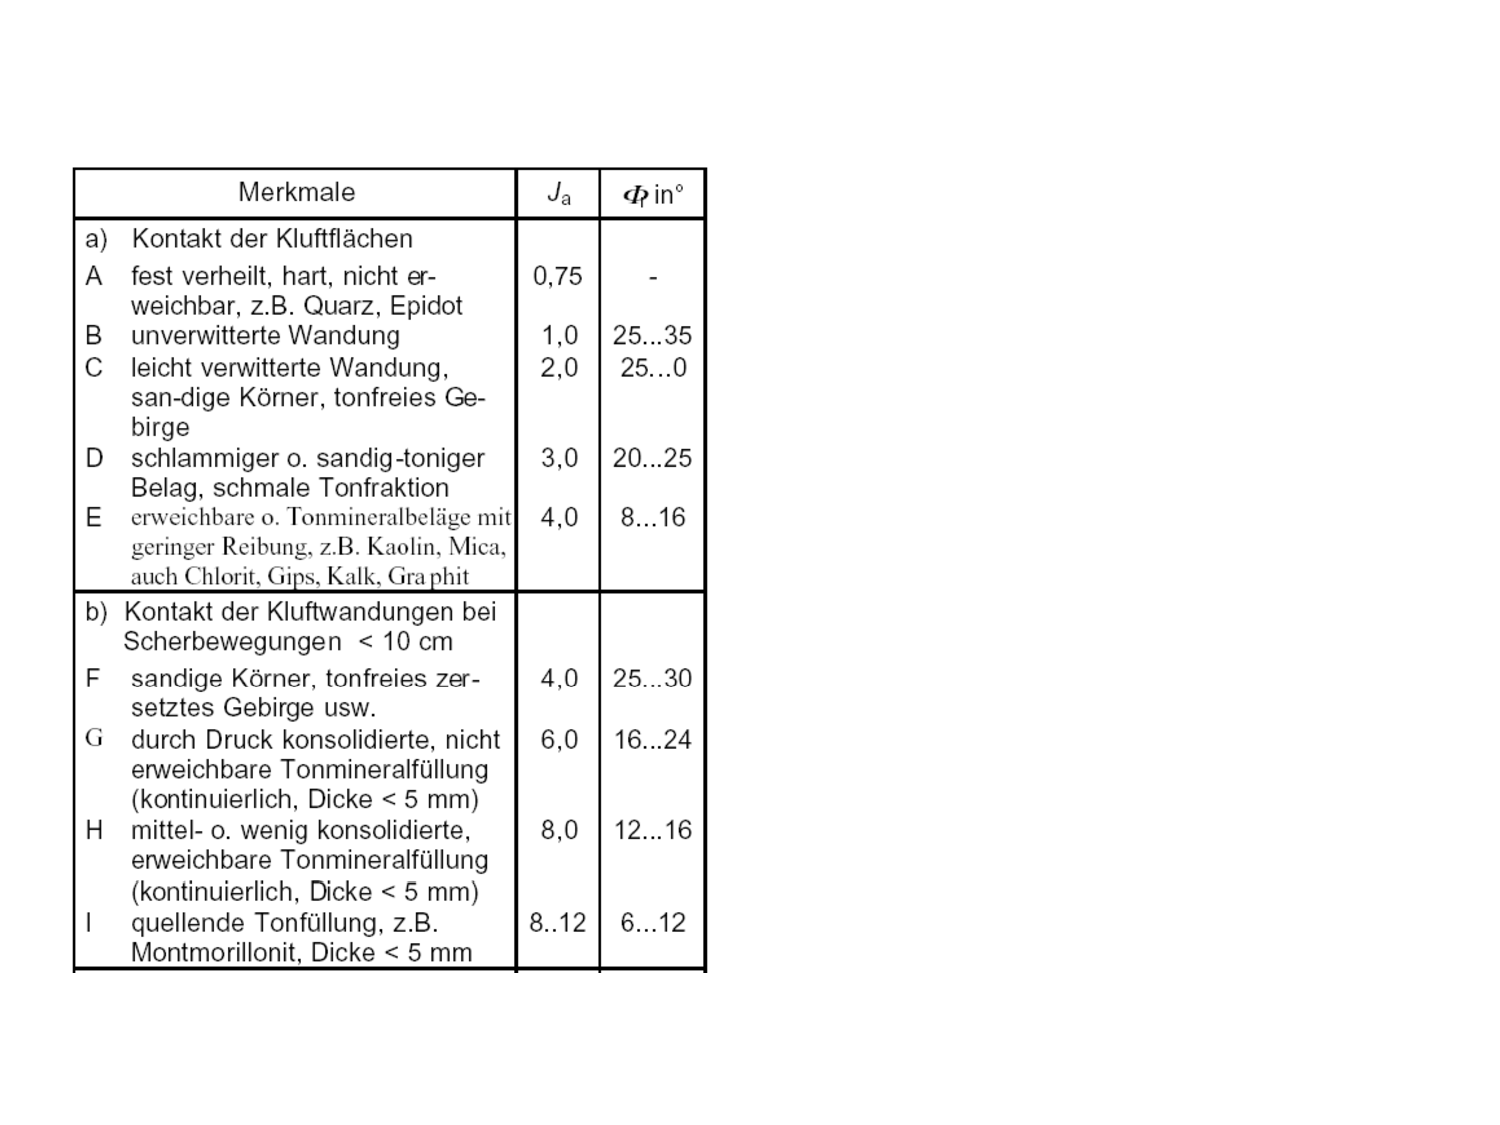
\includegraphics[width=0.8\textwidth]{Grafiken/J_aa.pdf}
\end{minipage}
\begin{minipage}{0.5\textwidth}
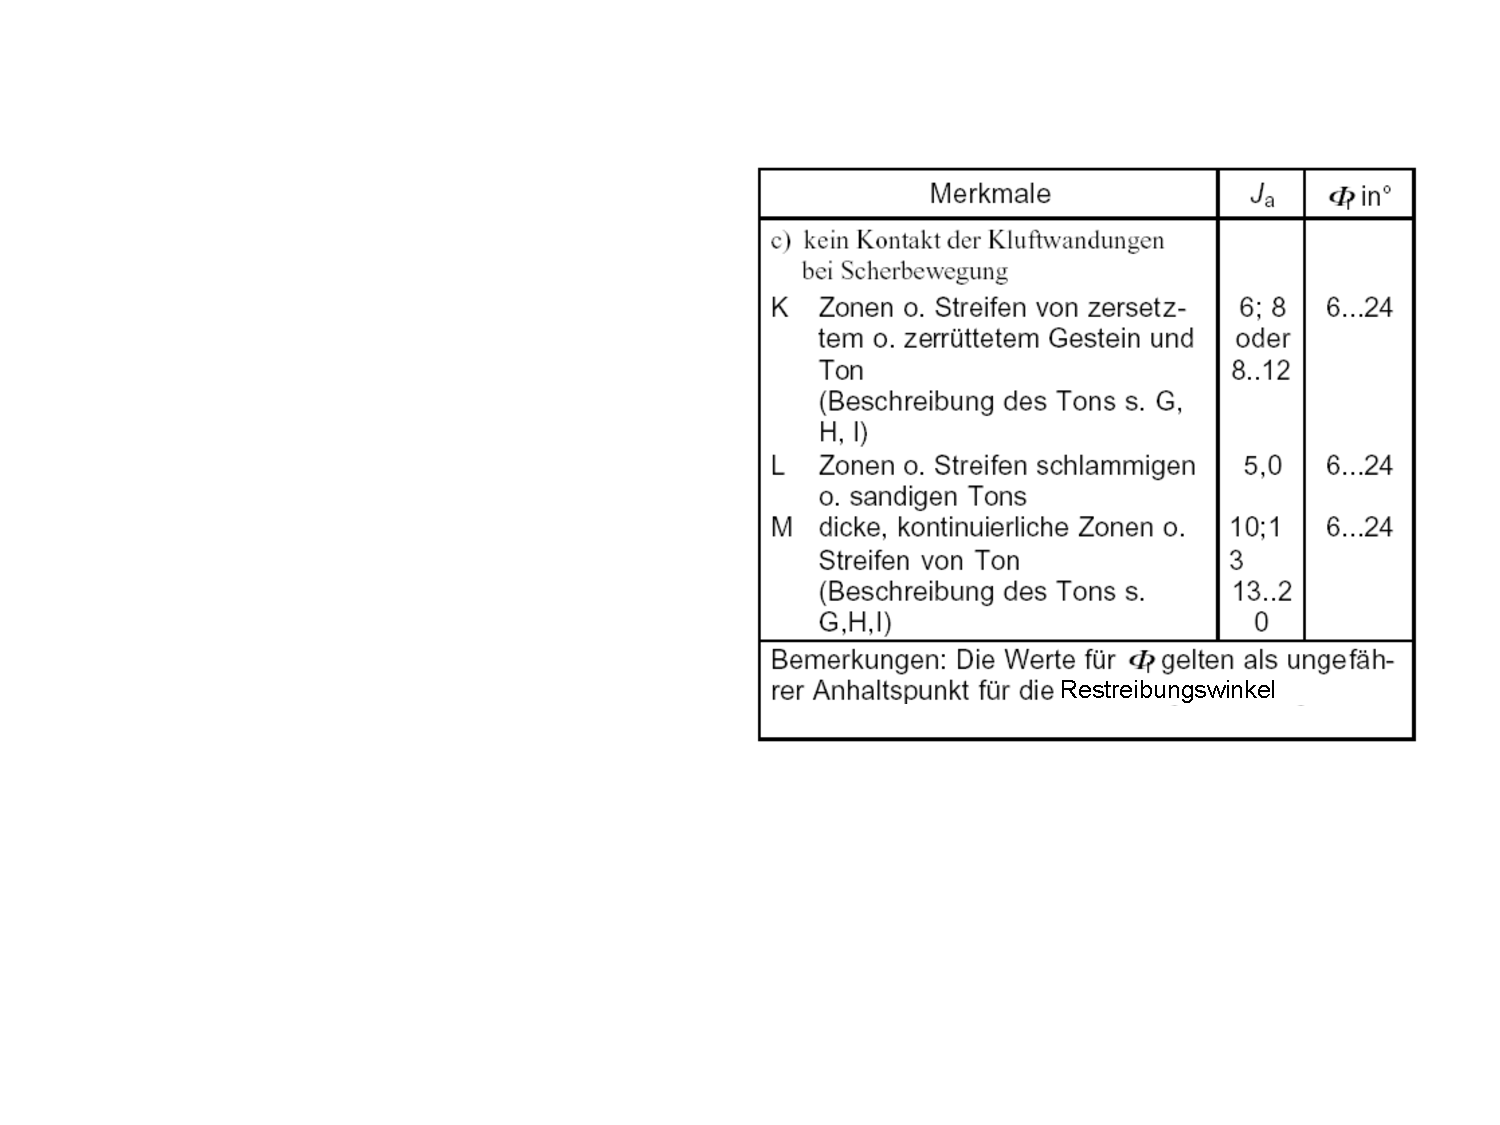
\includegraphics[width=0.8\textwidth]{Grafiken/J_ab.pdf}
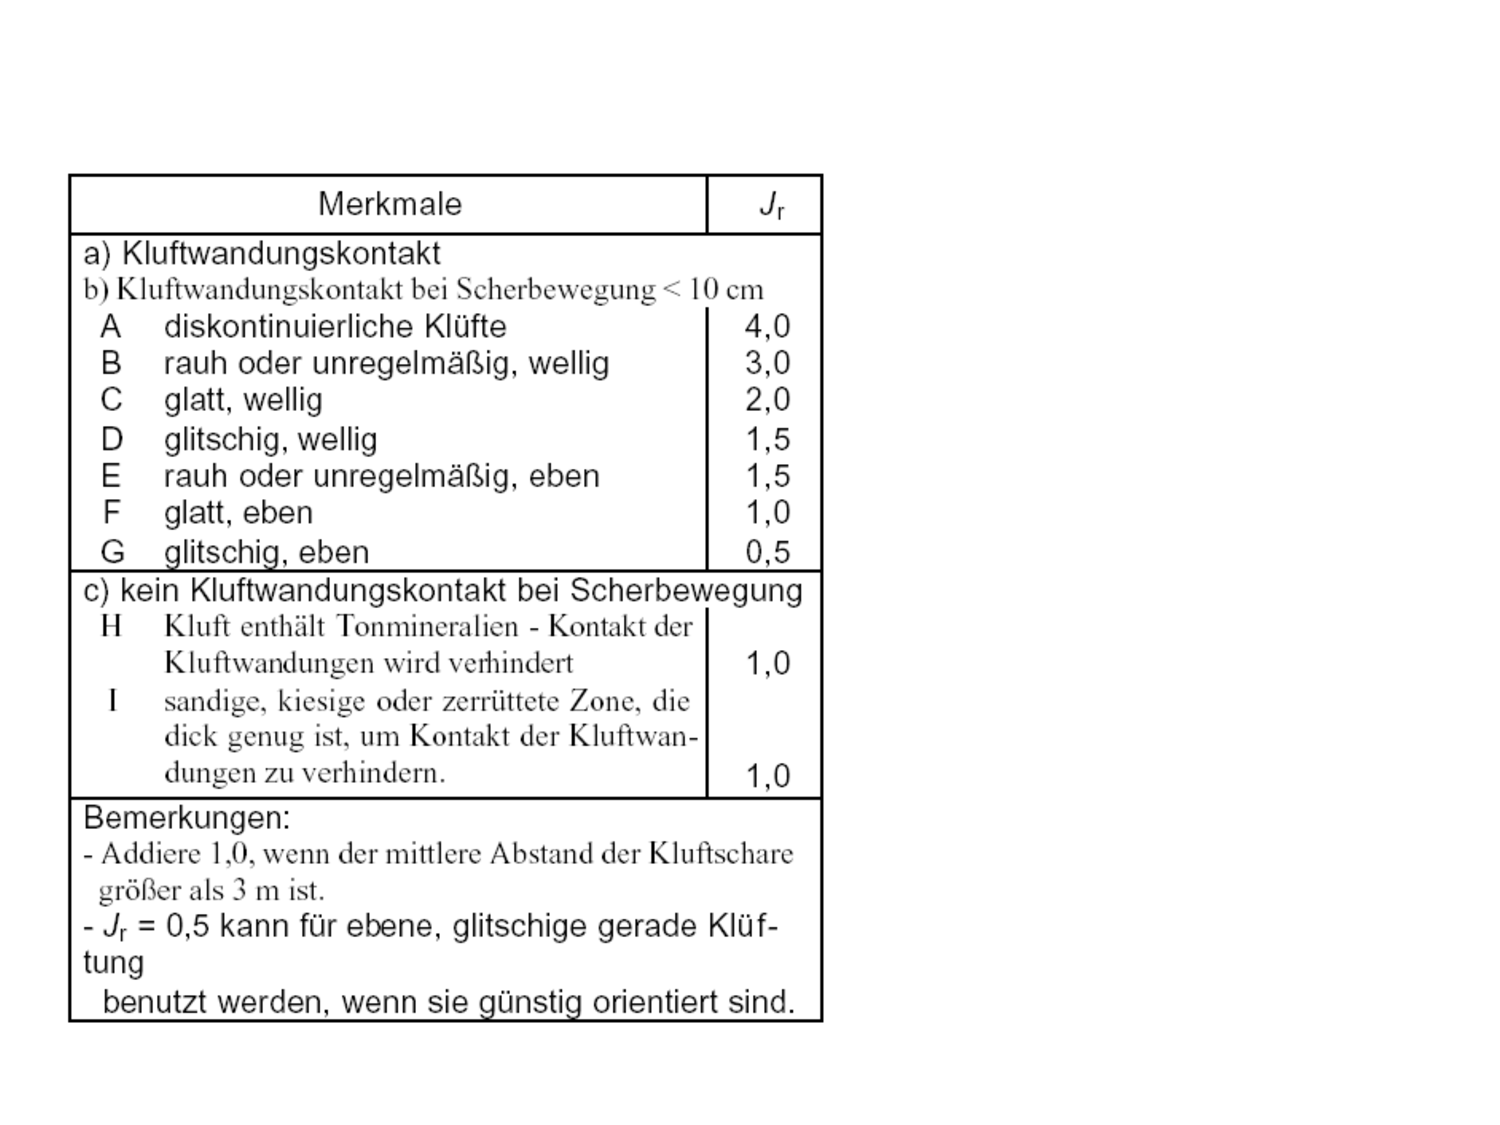
\includegraphics[width=0.8\textwidth]{Grafiken/J_r.pdf}
\end{minipage}
\begin{minipage}{0.5\textwidth}
    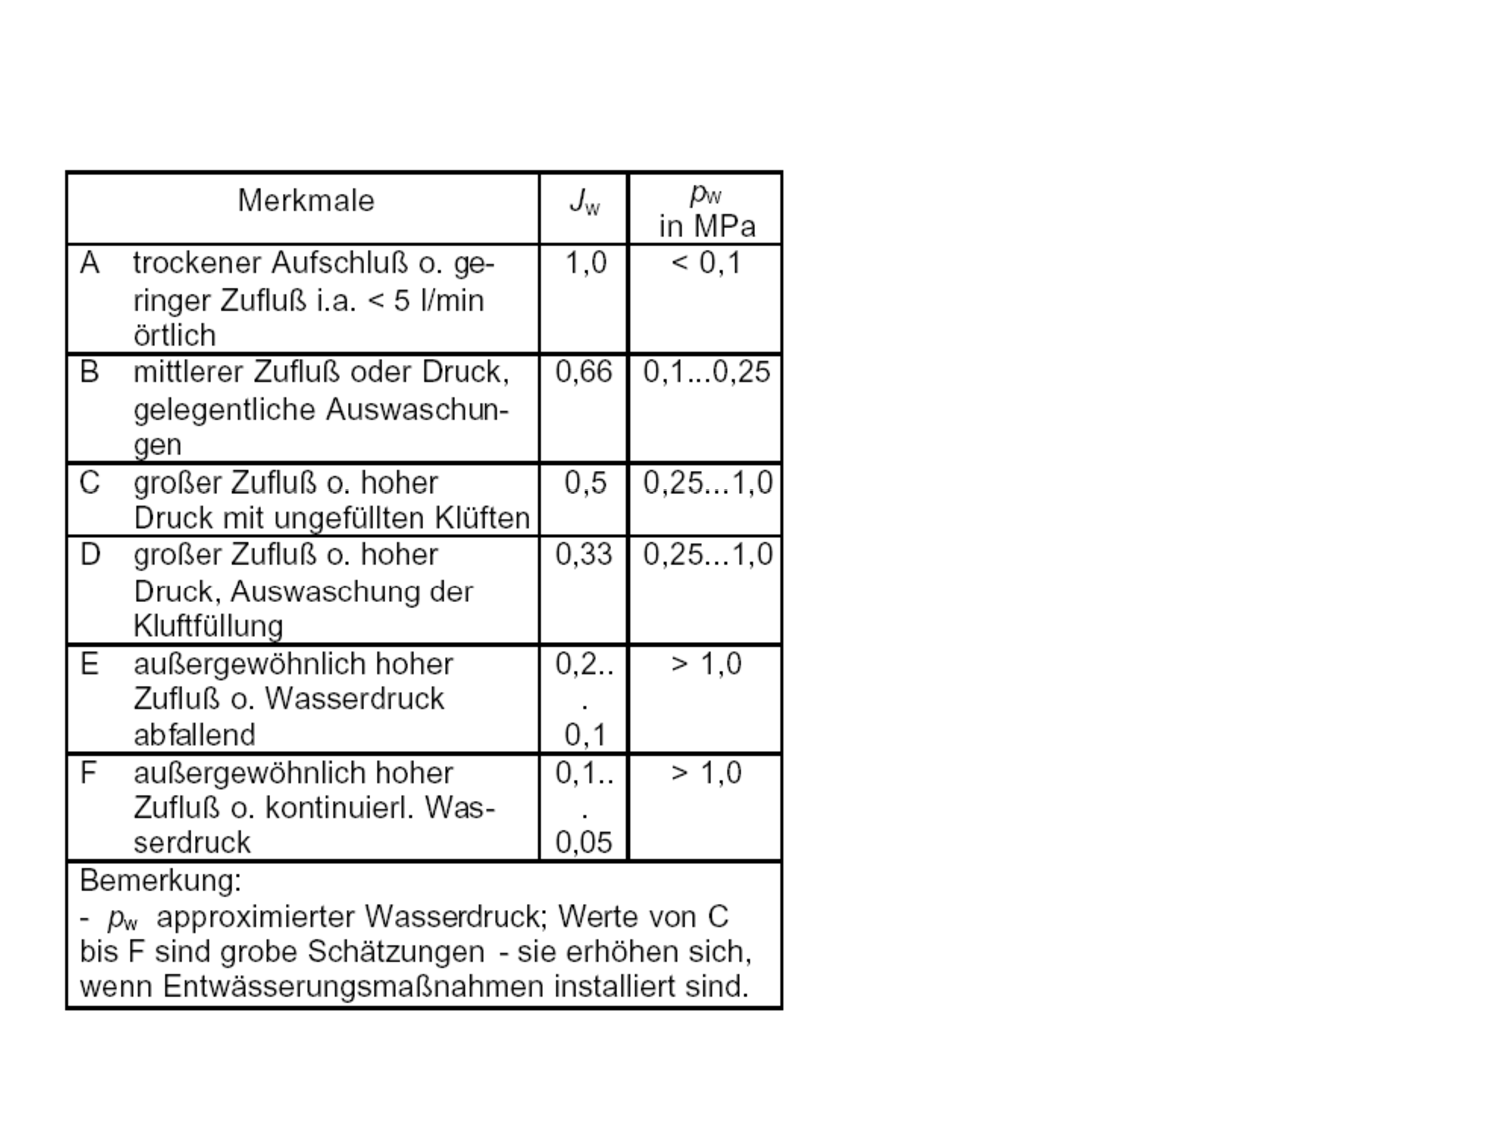
\includegraphics[width=0.8\textwidth]{Grafiken/J_w.pdf}
\end{minipage}
\begin{minipage}{0.49\textwidth}
    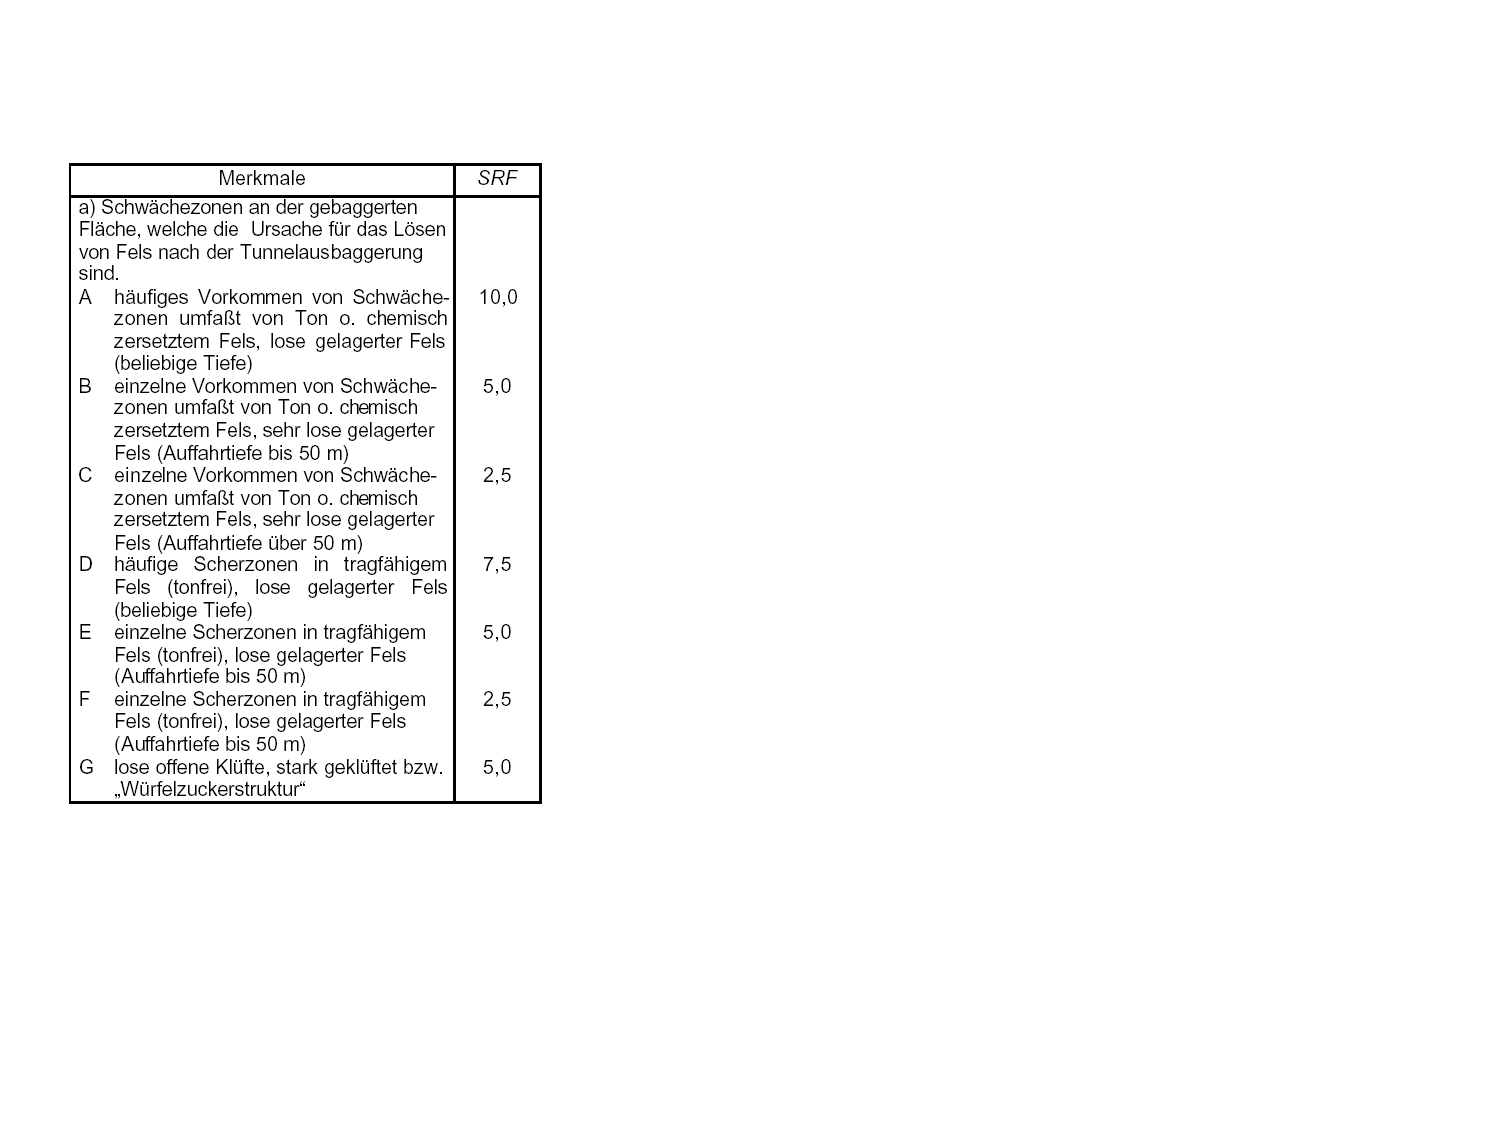
\includegraphics[width=0.8\textwidth]{Grafiken/SRFa.pdf}
\end{minipage}
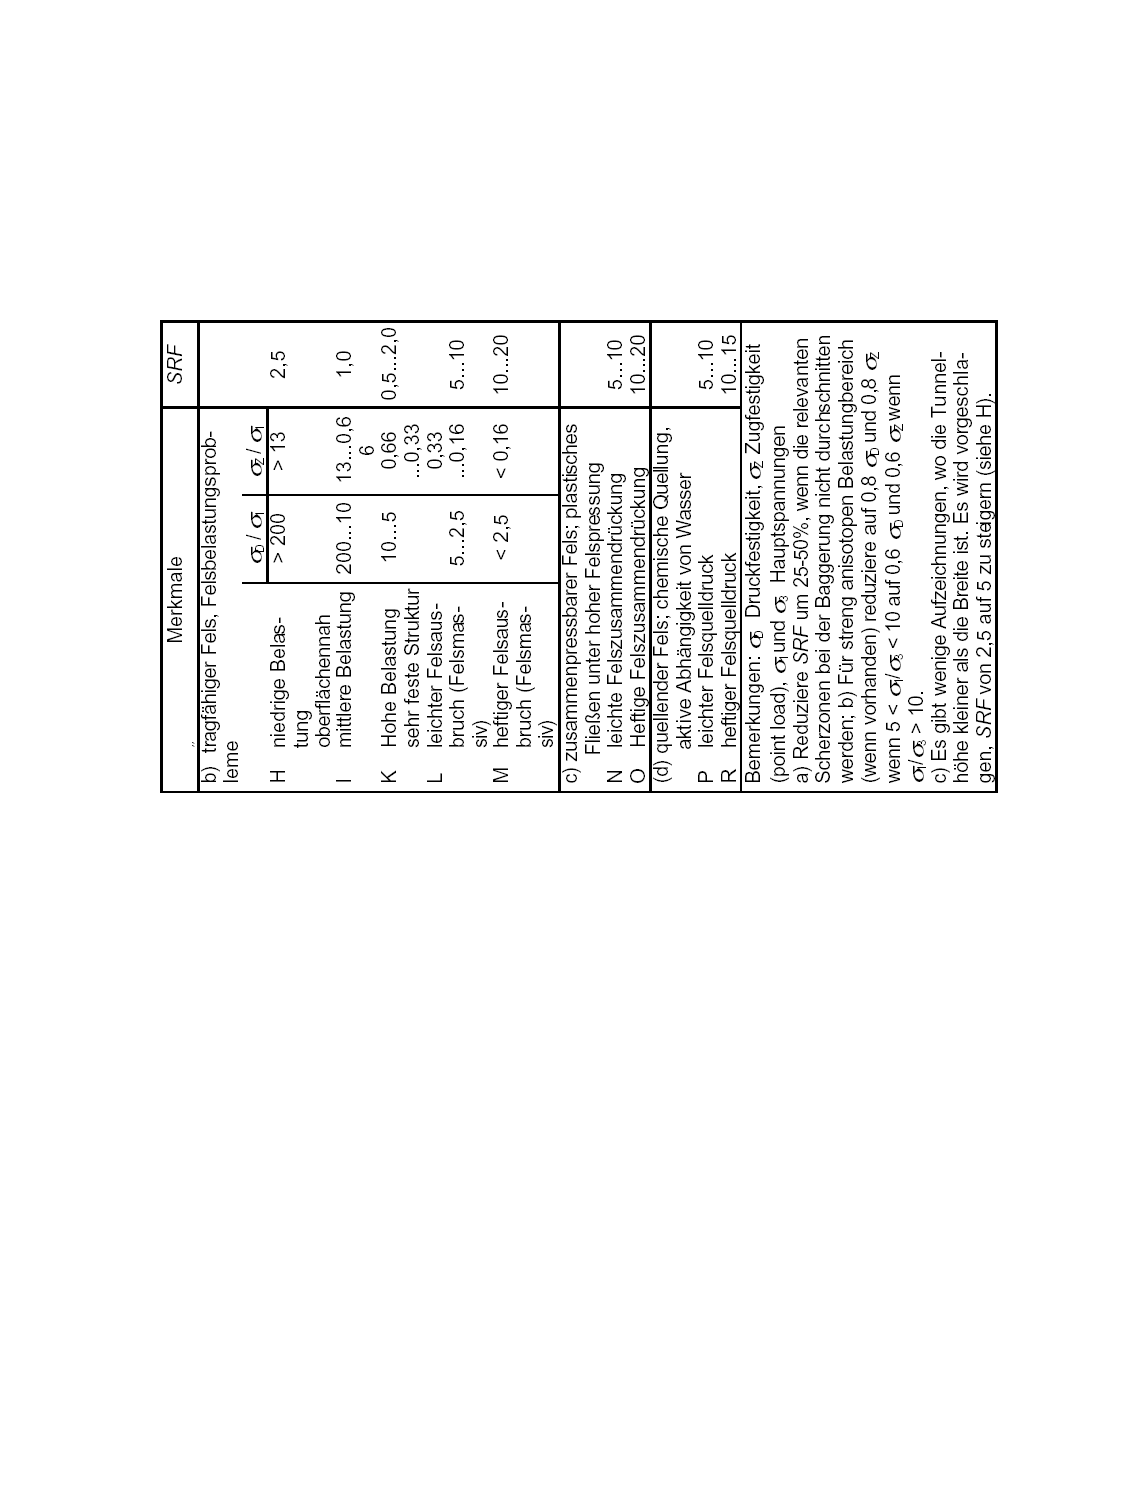
\includegraphics[width=0.8\textwidth]{Grafiken/SRFb.pdf}
\subsection{Berechnungsansätze}

\subsubsection{Theorie der gelochten Scheibe nach Kirsch}
\begin{minipage}{0.72\textwidth}
\begin{itemize}
    \item $\sigma_v = \gamma_{Geb} \cdot z$
    \item $\sigma_h = \lambda \cdot \sigma_v$ ; $\lambda = \frac{\nu}{1-\nu}$ ($0<\nu<0,5$); ($\nu =\frac{\text{Radiale Dehnung}}{\text{Axiale Dehnung}}$) Seitendruckbeiwert
    \item Radienverhältnis: $a=\frac{r_i}{r}$
    \item $\sigma_r = \frac{\sigma_v}{2}\left[(1+\lambda)\cdot(1-a^2)-(1-\lambda)\cdot(1-4a^2+3a^4)\cdot \cos(2\theta)\right] \overset{\wedge}{=} \sigma_3$
    \begin{itemize}
        \item Für $a=1$ (Hohlraumrand) $\sigma_{r}=0$
    \end{itemize}    \item $\sigma_\theta = \frac{\sigma_v}{2}\left[(1+\lambda)\cdot(1+a^2)+(1-\lambda)\cdot(1+3a^4)\cdot \cos(2\theta)\right] \overset{\wedge}{=} \sigma_1$
    \begin{itemize}
        \item Für $a=1$ (Hohlraumrand) $\sigma_{\theta}=\sigma_v[(1+\lambda)+2(1-\lambda)\cos(2\theta)]$
    \end{itemize}
    \item $\tau_{r\theta} = \frac{\sigma_v}{2}\left[ (1-\lambda)\cdot(1+2a^2-3a^4)\cdot \sin(2\theta) \right]$ (Treibende Spannung)
    \item Rahmenbedingungen: $\left\{
    \begin{tabular}{ p{1cm} p{0.2cm} c }
         $\lambda=0$ & $\Rightarrow$ & $-\sigma_v \leq \sigma_\theta \leq 3 \sigma_v$  \\
         $\lambda=1$ & $\Rightarrow$ & $\sigma_\theta \overset{!}{=} 2\sigma_v$ \\
    \end{tabular}
    \right. $
    \item Bei Klüften min/max mit $\theta=0^\circ/90^\circ$ berechnen und bei $v=\theta-\alpha_{Kluft}$ antragen.
\end{itemize}
\end{minipage}
\begin{minipage}{0.27\textwidth}
    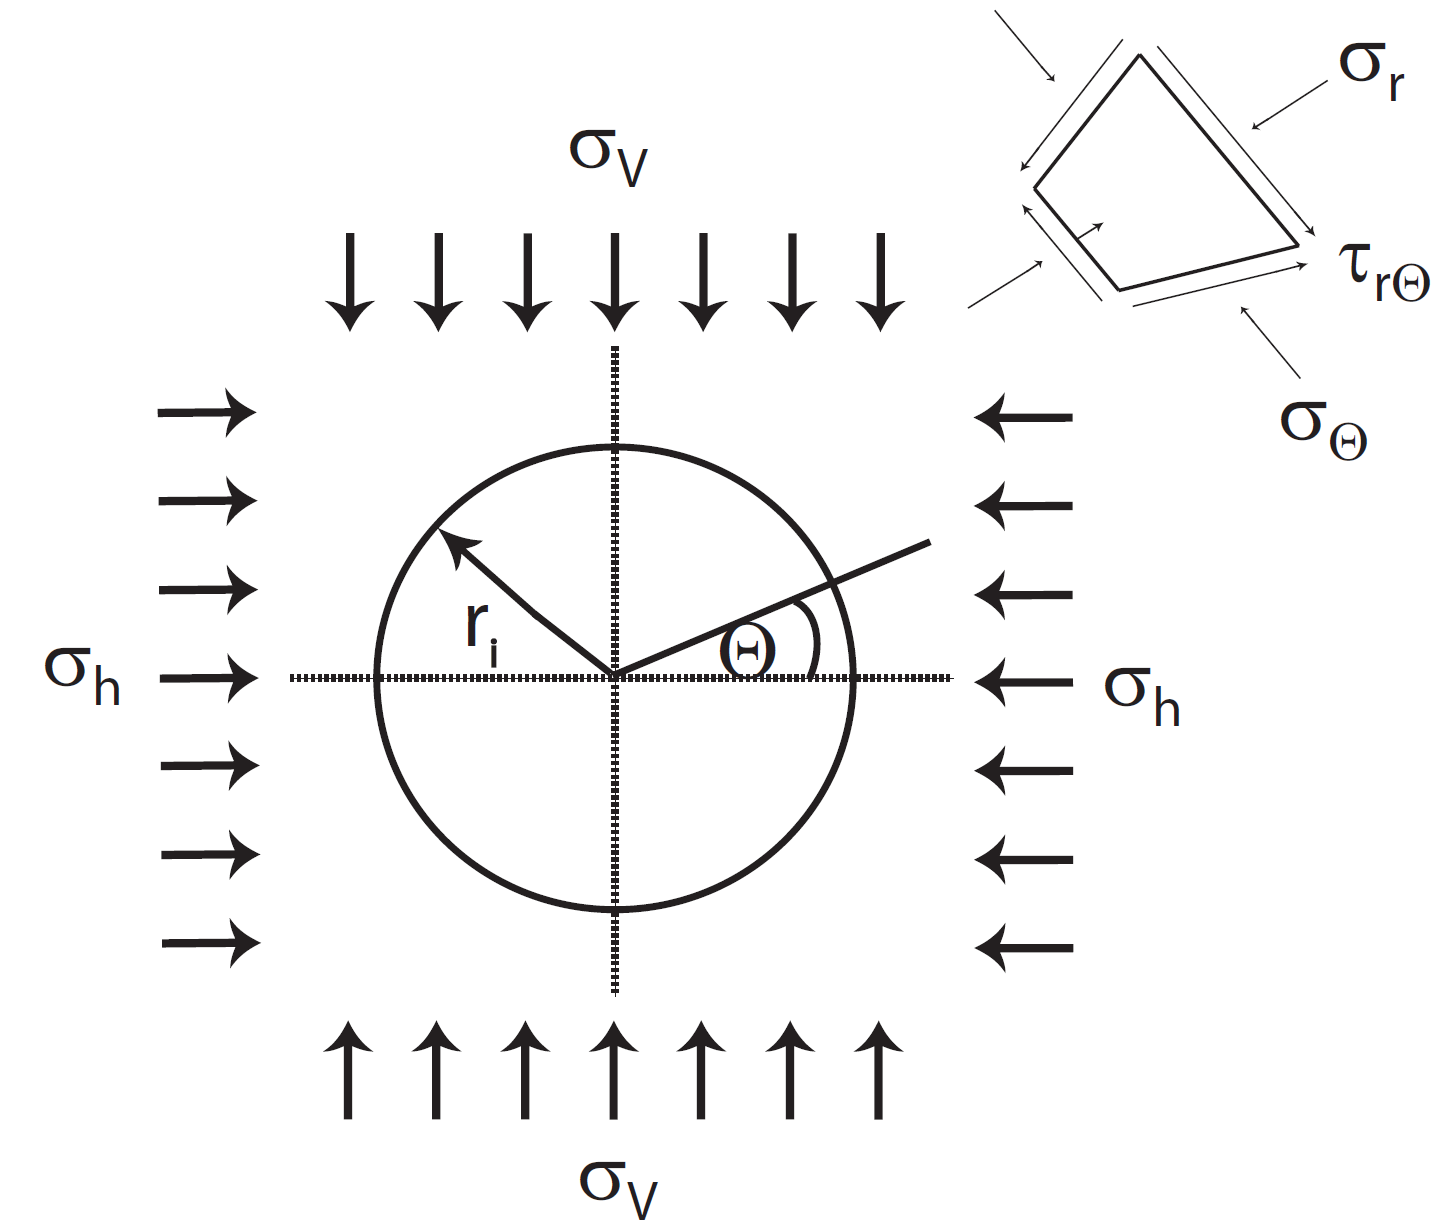
\includegraphics[width=1\textwidth]{Grafiken/gelochte Scheibe.png}
\end{minipage}


\subsubsection{Kreistunnel biaxialen Spannungen - Verschiebung des Hohlraumrandes}
\begin{minipage}{0.72\textwidth}
\begin{itemize}
	\item $u_r = \frac{\sigma_v(1+v)\cdot a\cdot r_i}{2\cdot E}[(1+\lambda)-(1-\lambda)\cdot(4\cdot(1-\nu)-a^2)\cdot\cos(2\theta)]$
	\item $u_\theta = \frac{\sigma_v(1+v)\cdot a\cdot r_i}{2\cdot E}(1-\lambda)\cdot[2\cdot(1-2\nu)+a^2]\cdot \sin(2\theta)$
	\item $u_{r,Ulme}=\frac{\sigma_v \cdot r_i}{E}(1+\nu)\cdot[1-2\cdot(1-\lambda)\cdot(1-\nu)]$
	\item $u_{r,Firste}=\frac{\sigma_v \cdot r_i}{E}(1+\nu)\cdot[\lambda+2\cdot(1-\lambda)\cdot(1-\nu)]$
\end{itemize}
\end{minipage}
\begin{minipage}{0.27\textwidth}
    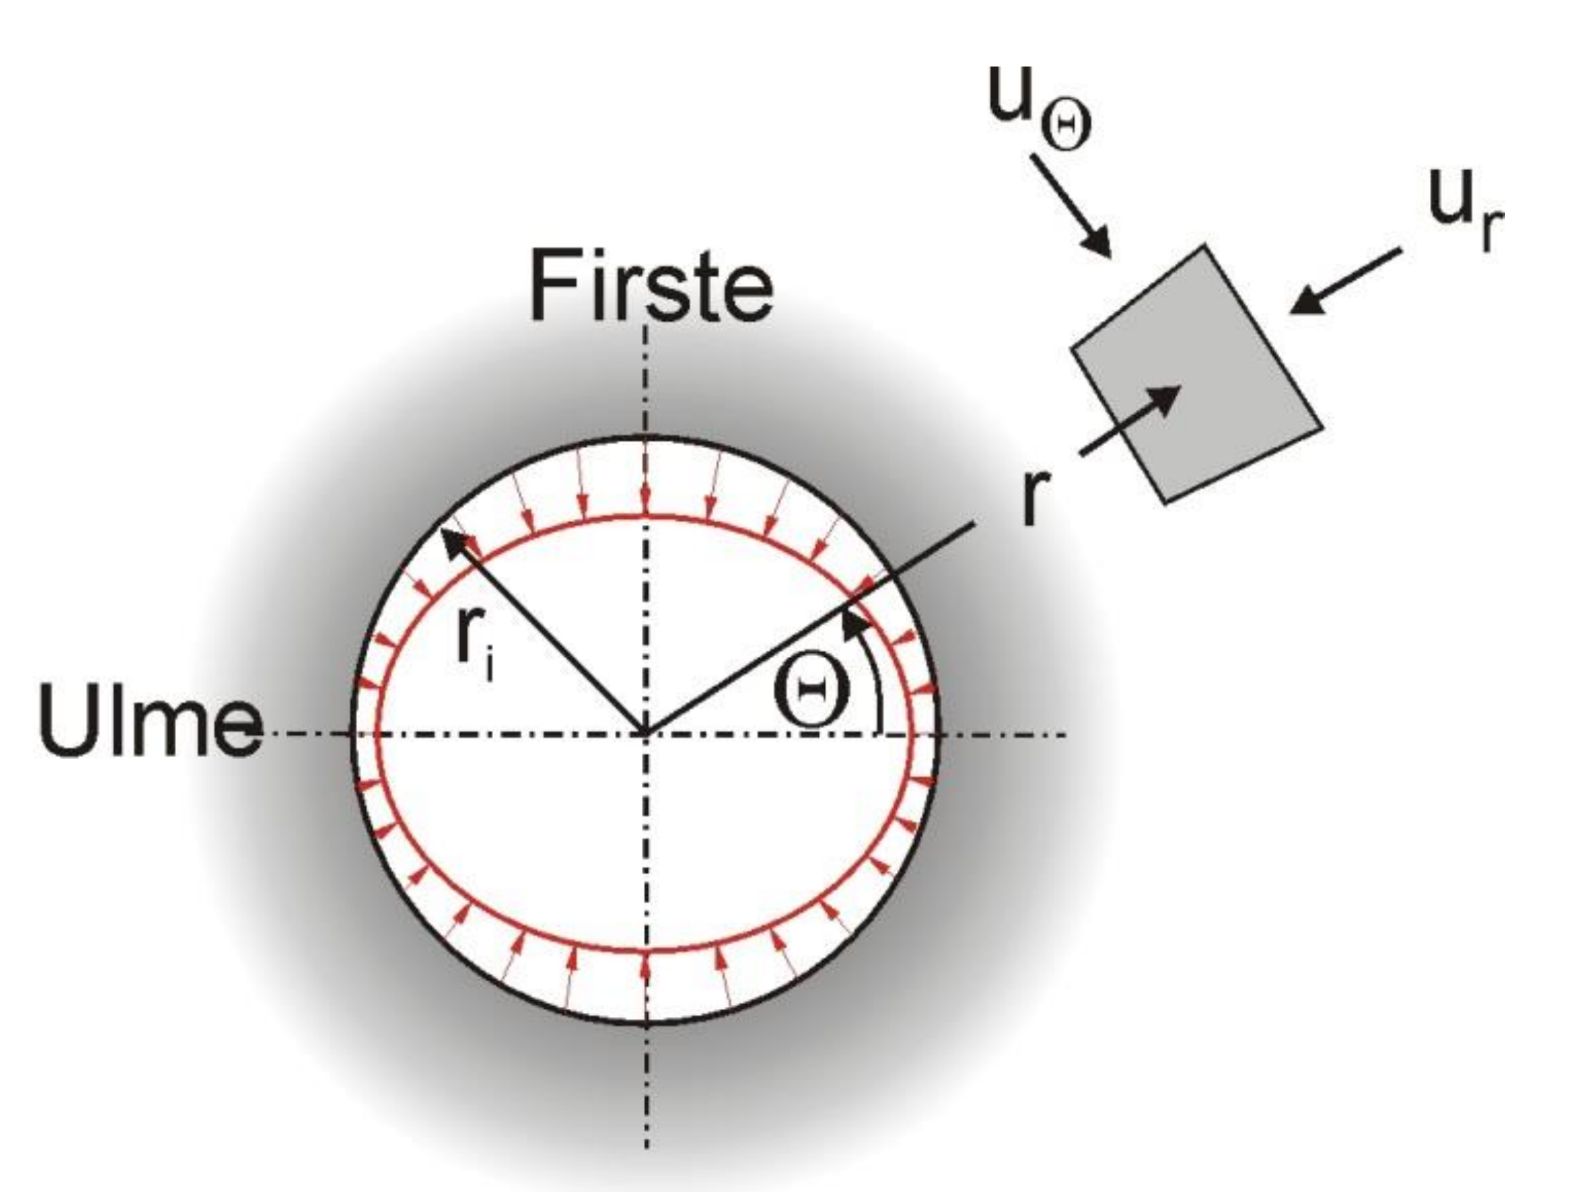
\includegraphics[width=0.99\textwidth]{Grafiken/Kreistunnel_biaxiale_Verschiebungen.png}
\end{minipage}

\subsubsection{Elliptischer Tunnelquerschnitt - Randspannungen}
\begin{minipage}{0.72\textwidth}
\begin{itemize}
    \item Höhe = 2h ; Breite = 2w
	\item $\sigma_r = 0$
	\item $\sigma_\theta = \sigma_v \cdot [(1+\lambda)-2\cdot (w-\lambda\cdot h)\cdot C]$
	\item $C=\dfrac{w \cdot \sin(\theta)^2-h\cdot \cos(\theta)^2}{w^2 \cdot \sin(\theta)^2 + h^2 \cdot \cos(\theta)^2}$
	\item Ulme: $\theta = 0^\circ , C = -\frac{1}{h} \Rightarrow \sigma_{\theta,Ulme} = \sigma_v \cdot \left[ 1+ 2 \cdot \frac{w}{h}-\lambda \right]$
	\item Firste: $\theta = 90^\circ , C = \frac{1}{w} \Rightarrow \sigma_{\theta,Firste} = \sigma_v \cdot \left[\lambda \cdot (1+2\cdot \frac{h}{w})-1 \right]$
\end{itemize}
\end{minipage}
\begin{minipage}{0.27\textwidth}
    \includegraphics[width=0.99\textwidth]{Grafiken/Elliptischer_tunnelquerschnitt_Randspannungen.png}
\end{minipage}
\begin{itemize}
    \item Sonderfälle:
    \begin{itemize}
        \item  $w = \lambda h$ $\Rightarrow$ $\sigma_\theta = \sigma_v (1+\lambda)$
        \item $w=h$ $\Rightarrow$ $\sigma_\theta \overset{\wedge}{=} $ \begin{footnotesize} Umfangsspannungen Kreistunnelwand bei biaxialen Primärspannungen \end{footnotesize}
        \item $w=h$ \& $\lambda = 1$ $\Rightarrow$ $\sigma_\theta = 2\sigma_v$ ; \begin{footnotesize} Umfangsspannungen Kreistunnelwand bei isotropen Primärspannungen \end{footnotesize}
    \end{itemize}
\end{itemize}

\subsubsection{Kreistunnel Spannungen im dickwandigen Rohr}
\begin{itemize}
    \item Radialspnnungen im dickwandigen Rohr: $\sigma_r=\frac{1}{\alpha-1}\left[-p_1\left(1-\left(\frac{r_2}{r}\right)^2\right)+p_2\left(\alpha-\left(\frac{r_2}{r}\right)^2\right)\right]$
    \begin{itemize}
        \item $\sigma_r=p_1$ wenn $r=r_1$; $\sigma_r=p_2$ wenn $r=r_2$
    \end{itemize}
    \item Tangentialspannung im dickwandigen Rohr: $\sigma_{\theta}=\frac{1}{\alpha-1}\left[-p_1\left(1+\left(\frac{r_2}{r}\right)^2\right)+p_2\left(\alpha+\left(\frac{r_2}{r}\right)^2\right)\right]$
    \item Tangentialspannung am Innenrand des dickwandigen Rohrs: $\sigma_{\theta}(r=r_1)=-p_1\frac{\alpha+1}{\alpha-1}+p_2\frac{2\alpha}{\alpha-1}$
    \begin{itemize}
        \item $\alpha=\left(\frac{r_2}{r_1}\right)^2$
        \item $r_1$: Innenradius Tunnelschale
        \item $r_2$: Ausbruchsradius
        \item $p_1$: Innendruck
        \item $p_2$: Außendruck
    \end{itemize}
\end{itemize}

\subsubsection{Kreistunnel im elasto-plastischen Gebirge}
\begin{itemize}
	\item Annahme: isotrope Primärspannungen $(\sigma_v = \sigma_h)$
	\item $\sigma_1 = \sigma_\theta \& \sigma_3 = \sigma_r$
	\item $\sigma_\theta = \sigma_r \frac{1+\sin\phi}{1-\sin\phi} + \frac{2c \cdot \cos\phi}{1-\sin\phi}$\\
	oder: $\sigma_\theta = \lambda_p \cdot \sigma_r + \sigma_u$
	\item $\lambda_p = \frac{1+\sin\phi}{1-\sin\phi}$ ; $\sigma_u = \frac{2c \cdot \cos\phi}{1-\sin\phi}$\\
	$\lambda_p$ = passiver Seitendruckbeiwert; $\phi$ = Reibungswinkel; $\sigma_u$ = einachsige Druckfestigkeit des Gebirges
\end{itemize}

\subsubsection{Kreistunnel im elasto-plastischen Gebirge - Werte in der plastischen Zone}
\begin{itemize}
	\item Das Gestein geht am Hohlraumrand zu Bruch, wenn gilt: $\sigma_\theta = \lambda_p \sigma_r + \sigma_u$
	\item Radialspannung: $\sigma_{r,pl} = \left( p_i + \frac{\sigma_u}{\lambda_p -1} \right) \cdot \left( \frac{r}{r_i} \right)^{\lambda_p -1} - \frac{\sigma_u}{\lambda_p -1}$
	\item Axialspannungen: $\sigma_{\theta,pl} = \lambda_p \cdot \left[ \left( p_i + \frac{\sigma_u}{\lambda_p -1} \right) \cdot \left( \frac{r}{r_i}\right)^{\lambda_p -1} - \frac{\sigma_u}{\lambda_p -1}\right] + \sigma_u$
	\item Druck ($r=r_{pl}$): $p_{pl} = \left( p_i + \frac{\sigma_u}{\lambda_p -1} \right) \cdot \left( \frac{r_{pl}}{r_i} \right)^{\lambda_p -1} - \frac{\sigma_u}{\lambda_p -1}$
	\item plastischer Radius: $r_{pl}=r_i \cdot \left[ \dfrac{p_{pl} +\frac{\sigma_u}{\lambda_p -1}}{p_i +\frac{\sigma_u}{\lambda_p -1}} \right]^{\frac{1}{\lambda_p -1}}$ oder $r_{pl} = r_i \left[ \dfrac{2}{1+ \lambda_p} \cdot \dfrac{\sigma_\infty \cdot (\lambda_p -1) + \sigma_u}{p_i \cdot (\lambda_p -1) + \sigma_u} \right]^{\frac{1}{(\lambda_p -1)}}$\\
	Für $p_i=0$ gilt dann $r_{pl}=r_i\left[\frac2{1+\lambda_p}\left(\frac{\sigma_{\infty}}{\sigma_u}(\lambda_p-1)+1\right)\right]^{\frac{1}{\lambda_p-1}}$
	\begin{itemize}
	    \item Einaxiale Druckfestigkeit: $\sigma_u=\frac{2c\cos(\varphi)}{1-\sin(\varphi)}$
	    \item Fernfeldspannung: $\sigma_{\infty}:$
	    $\left\{
    \begin{tabular}{ p{2.5cm} p{0.2cm} c }
         Vor Ausbruch & $\Rightarrow$ & $\sigma_{\infty} = \sigma_h \text{ bzw. } \sigma_v$  \\
         Nach Ausbruch & $\Rightarrow$ & $\sigma_\theta(0^\circ-90^\circ)$ \\
    \end{tabular}
    \right. $
	\end{itemize}
	\item $\sigma_r = \sigma_\infty \left( 1-\left( \frac{r_{pl}}{r}\right) ^2 \right) + p_{pl} \left(\frac{r_{pl}}{r}\right)^2$
	\item $\sigma_\theta = \sigma_\infty \left( 1+\left( \frac{r_{pl}}{r}\right) ^2 \right) - p_{pl} \left(\frac{r_{pl}}{r}\right)^2$
\end{itemize}

\subsubsection{Hoek-Brown'sches Versagenskriterium}

\begin{itemize}
    \item $\sigma_1=\sigma_3+\left(m\sigma_c\sigma_3+s\sigma_c^2\right)^a$
    \item $\dfrac{\sigma_t}{\sigma_c}=\frac12\left(\sqrt{m_i^2+4}-m_i\right)$
    \begin{itemize}
        \item Böschungen und durch Sprengen beschädigte Ausbrüche: $m=m_ie^{\frac{RMR-100}{14}}$
        \item Böschungen und durch Sprengen beschädigte Ausbrüche: $s=e^{\frac{RMR-100}{6}}$
        \item Gebirgsschonend: $m=m_ie^{\frac{RMR-100}{28}}$ %=\frac{\sigma_c}{\sigma_t}-\frac{\sigma_t}{\sigma_c}$
        \item Gebirgsschonend: $s=e^{\frac{RMR-100}{9}}$\\$s=1$ für intakten Fels
        \begin{itemize}
            \item $m_i=7$ für Karbonatgesteine
            \item $m_i=10$ für verfestigte tonige Gesteine
            \item $m_i=15$ für sandhaltige Gesteine
            \item $m_i=25$ für grobkörnige polimineralische magmatische oder metamorphe Gesteine
        \end{itemize}
        \item $a=\frac12+\frac16e^{-\frac{GSI}{15}}-e^{\frac{-20}{3}}$ i.d.R. $a=0,5$
        \item $\sigma_{ti}$ siehe \autoref{Spaltzugversuch}
        \item $\sigma_{ci}$ siehe \autoref{Punktlastversuch}
    \end{itemize}
    \item Einaxiale Druckfestigkeit der Felsmasse $\sigma_c=\sigma_{ci}s^a$
    \item Zugfestigkeit der Felsmasse $\sigma_t=\frac{s\sigma_{ci}}{m}$
\end{itemize}

\subsubsection{Fließkriterium nach Drucker-Prager}

    \begin{itemize}
        \item Das Fließkriterium nach Drucker–Prager ist für Polymere, für Böden und für granulare Stoffe geeignet.
        \item $\sigma_v = \frac{m-1}{2}(\sigma_1 + \sigma_2 + \sigma_3) + \frac{m+1}{2} \sqrt{\frac{1}{2} \left[ (\sigma_1 - \sigma_2)^2 + (\sigma_2 - \sigma_3)^2 (\sigma_3 - \sigma_1)^2 \right] }$
        \item $m = \frac{\sigma_c}{\sigma_t}$
        \item $\sigma_c$: Grenzspannung für Druck
        \item $\sigma_f$: Grenzspannung für Zug
        \item Die Besonderheit dieser Vergleichsspannung ist, dass wie beim Fließkriterium nach Mohr-Coulomb zwischen Druck- und Zugspannungen unterschieden wird. Das Verhältnis der Grenzspannungen von Druck und Zug geht in die Ermittlung der Vergleichsspannung ein.
        \item Sind $\sigma_c$ und $\sigma_f$ gleich, dann wird daraus die Von-Mises-Vergleichsspannung. Die Gestaltänderungsenergiehypothese ist also ein Sonderfall des Fließkriteriums nach Drucker-Prager.
    \end{itemize}
  
  
\subsection{Nachweise}

\subsubsection{Standsicherheit des Tunnels}
\begin{itemize}
    \item Nur in axialer Richtung betrachtet: $\sigma_\theta > \sigma_u \Rightarrow$ Versagen findet statt
    \item $\sigma_u = \frac{2c \cdot \cos(\varphi)}{1-\sin(\varphi)}$ ; einachsige Druckfestigkeit Gebirge
\end{itemize}


\subsubsection{Standsicherheit mit Innendruck}
\begin{itemize}
    \item Versagen tritt ein: $\sigma_{\theta} > \sigma_1 = (s \sigma_c^2)^{\frac12}$
    \item Bei einem Innendruck $p$ gilt: $\sigma_r=p$ $\&$ $\sigma_\theta=2\sigma_v-p$
    \item Versagensbedigung: (Gleich 0 setzen und auflösen)\\
    $\sigma_1 = \sigma_3 + (m\sigma_c\sigma_3+s\sigma_c^2)^\frac12 \\
    2\sigma_v-p=p+(m\sigma_cp+s\sigma_c^2)^{\frac12}$ $\Rightarrow$ $p$ 
    \item Allgemeiner Ansatz: $\sigma_{\theta}-p_i = \lambda_p \cdot p + \sigma_u$
    \begin{itemize}
        \item $\sigma_u$ für Mohr-Coulomb mit $\sigma_{u(\text{Intakt})}$ und für John'schen mit $\sigma_{u,(\text{Klüfte})}$
        \item $\lambda_{pi,(\varphi_i)}$ oder $\lambda_{pk,(\varphi_k)}$
    \end{itemize}
\end{itemize}

\subsubsection{Ort versagen Tunnelwandung}
\begin{itemize}
    \item $\varphi_{crit}=45+\frac{\varphi}{2}$
    \item Tunnelrand: $\sigma_r=0 \Rightarrow \sigma_3 = 0$
    \item Einaxiale Auswertung:
    \begin{itemize}
        \item  Einwirkung: $\sigma_\theta$ für $0^\circ/90^\circ$
        \item Widerstand:$\sigma_{(\text{Klüfte})}=\dfrac{\sigma_3\left[\sin(2\alpha_k-\varphi_k)+\sin(\varphi_k)\right]+2c_k\cos(\varphi_k)}{\sin(2\alpha_k-\varphi_k)-\sin(\varphi_k)}$ ; $\sigma_{(\text{Fels})} = \dfrac{2c \cdot \cos(\varphi)}{1-\sin(\varphi)}$
    \end{itemize}
    \item Gleichsetzen und nach $\theta$ auflösen ($\alpha=Kluftwinkel+\theta$)
\end{itemize}

\subsubsection{Seitendruckbeiwert und Wasserdruck}
\begin{itemize}
    \item Bei welchem Seitendruckbeiwert des Tunnels wird die vertikale Auflast maximal?\\
    $\blacktriangleright$ Seitendruckbeiwert so wählen, dass Normalkraft genau durch Wasser aufgehoben ist. Dadurch keine Reibungskräfte und der Keil würde von alleine abgleiten.\\
            $W=N$ $\Rightarrow$ $W=0,5\cdot \gamma_w \cdot h^2 \cdot \lambda_w = N = 0,5 \cdot \gamma \cdot h^2 \cdot \lambda$
\end{itemize}


\subsubsection{Standsicherheit Keil}
\begin{minipage}{0.72\textwidth}
\begin{itemize}
	\item $\psi$ = Gleitwinkel auf dem Keil abrutscht
	\item Gewicht Keil: $W = \gamma \cdot A$
	\item Standsicherheitsfaktor: $\nu = \dfrac{c \cdot I + W\cos(\psi) \tan(\phi)}{W \sin(\psi)} \overset{!}{\geq} 1$\\
        l = Länge Gleitfläche
    \item Standsicherheitsfaktor mit Anker:\vspace{5pt}\\
    $\nu = \dfrac{c \cdot I + (W\cos(\psi) + T\cos(\theta))\tan(\phi) +T\sin(\theta)}{W \sin(\psi)}$\\
    $T$ = Ankerkfraft
\end{itemize}
\end{minipage}
\begin{minipage}{0.27\textwidth}
    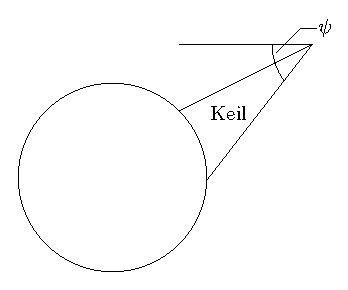
\includegraphics[width=0.99\textwidth]{Grafiken/Abrutschen_Keil.eps}
\end{minipage}

\subsubsection{Stützung der Bohrlochwandung mit Suspension}
\begin{itemize}
    \item In-situ Spannungszustand: $\sigma_v$ $\&$ $\sigma_h$
    \item $\sigma_{\theta\theta}\text{(Ulme)} = \sigma_v(3-\lambda)$ ; $\sigma_{\theta\theta}\text{(Firste)} = \sigma_v(3\lambda-1)$
        \begin{itemize}
            \item Sonderfall: Vertikale Bohrung mit Suspensionsstützung: $\lambda=1$, also gilt $\sigma_{\theta\theta}=2\sigma_h$
        \end{itemize} 
    \item Spannungszustand Ulme: $\sigma_{rr}=p \overset{\wedge}{=}  \sigma_1$ ; $\sigma_{\theta\theta}(Ulme) \overset{\wedge}{=} \sigma_{3/h}$
    \item Minimaler hydraulischer Druck Ulme ($\sigma_{rr} < \sigma_{\theta\theta}): \sigma_{rr}$ bzw. $p$ nach Mohr-Coulomb.
        \begin{itemize}
            \item Falls: $\sigma_{\theta\theta}-p>0$ treten mit Bohrspülung keine Zugspannungen auf und Stützung mit Suspension ist möglich.
        \end{itemize}
    \item Berechnung Wichte der Suspension: $\gamma_s \cdot z = p$
\end{itemize}

\subsubsection{In welchem Bereich darf Wichte der Suspension liegen? (kein Versagen)}
\begin{itemize}
    \item Mindestwasserdruck: $\sigma_{\theta,horizontal}-p=\lambda_p \cdot p +\sigma_u$ $\Rightarrow$ nach p auflösen
    \item Maximalwasserdruck: $\sigma_{\theta,vertikal}-p=\sigma_t$ $\Rightarrow$ nach p auflösen
\end{itemize}


\subsubsection{Gleichmäßiges Kammer- Pfeiler System}
\begin{minipage}{.52\textwidth}
\begin{itemize}
    \item 2D Fall (Unendlich Lange Wände)
    \begin{itemize}
        \item Aubbauverlust: $r=\frac{w_p}{w_0+w_p}$
        \item Pfeilerspannung: $\sigma_p=\sigma_0\frac{w_0+w_p}{w_p}=\frac{\sigma_0}{r}$
        \item Nicht eingekleidete Pfeiler: $\sigma_p = \sigma(\sigma_3=0) $
    \end{itemize}
    \item 3D Fall (Rechteckige Pfeiler)
    \begin{itemize}
        \item Abbauverlust: $r=\frac{a\cdot b}{(a+c)(b+d)}$
        \item Pfeilerspannung: $\sigma_p\cdot a\cdot b=(a+c)(b+d)\cdot \sigma_v\\\Rightarrow\sigma_p=\frac{(a+c)\cdot (b+d)}{a\cdot b}\sigma_v=\frac{\sigma_v}{r}$
    \end{itemize}
    \item Skaleneffekt:\\Eigenschaften werden von Probengröße beeinflusst.
    \begin{itemize}
        \item $\sigma_c=\sigma_{c0}\left(\frac{V}{V_0}\right)^{-\frac{1}{m}}$
    \end{itemize}
\end{itemize}
\end{minipage}
\begin{minipage}{.47\textwidth}
    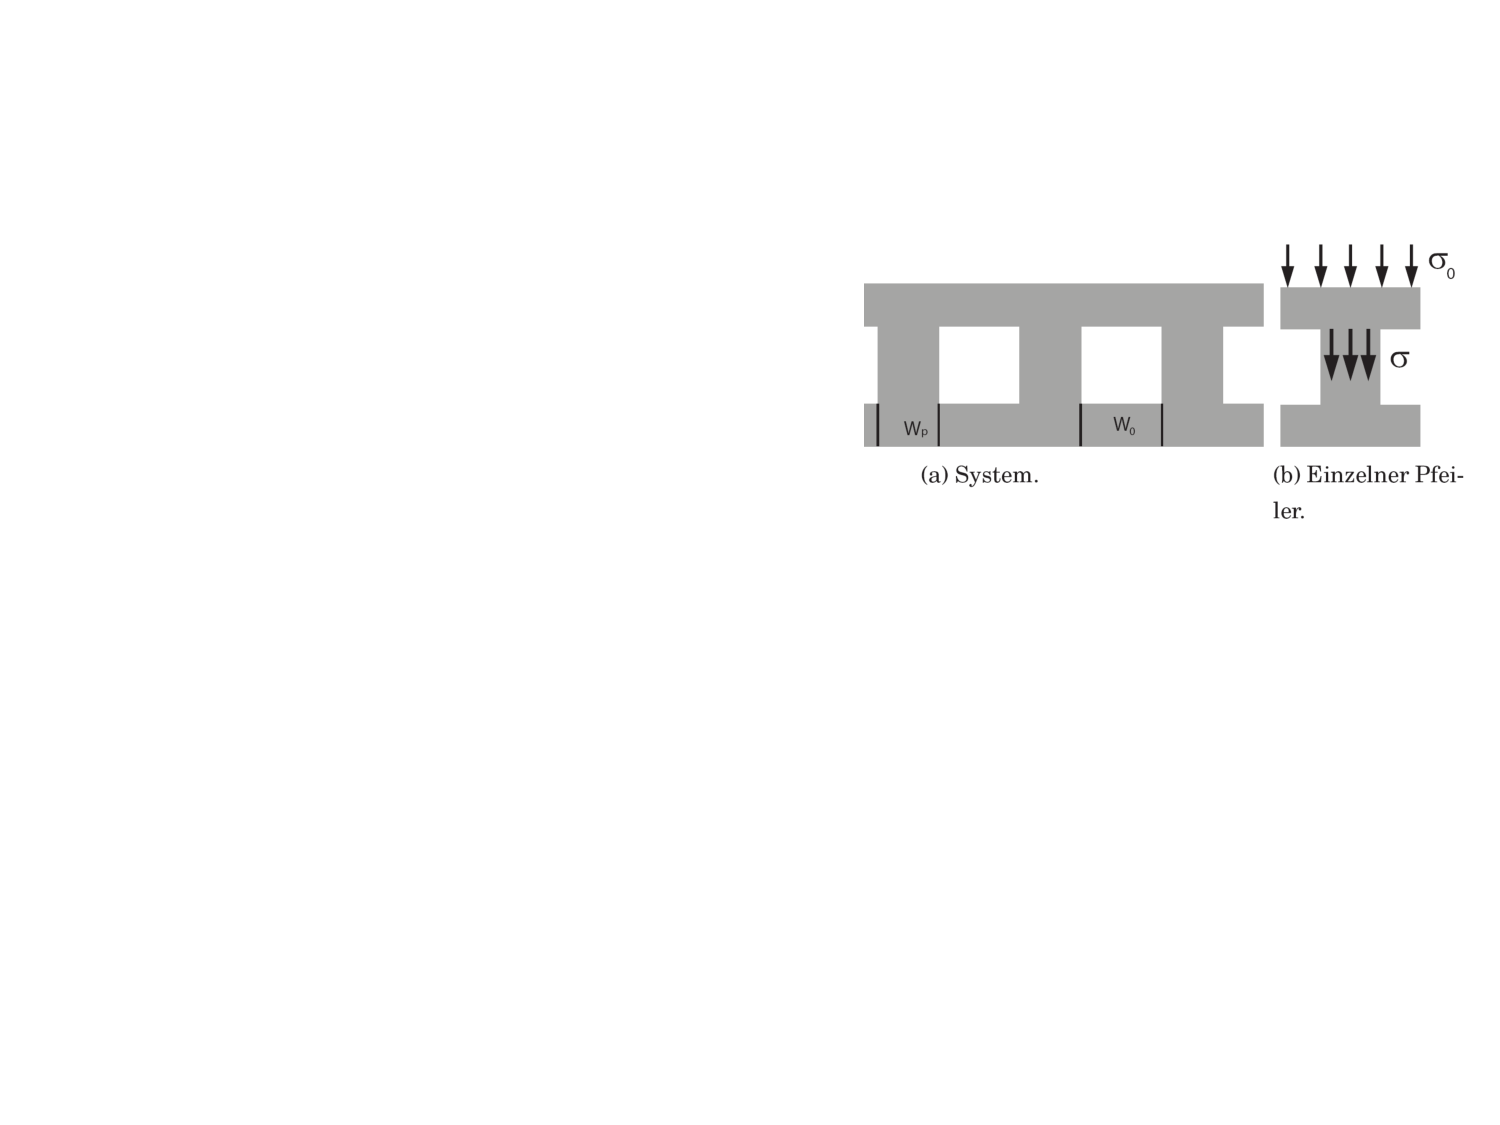
\includegraphics[width=0.8\textwidth]{Grafiken/Abbauverlust.pdf}
    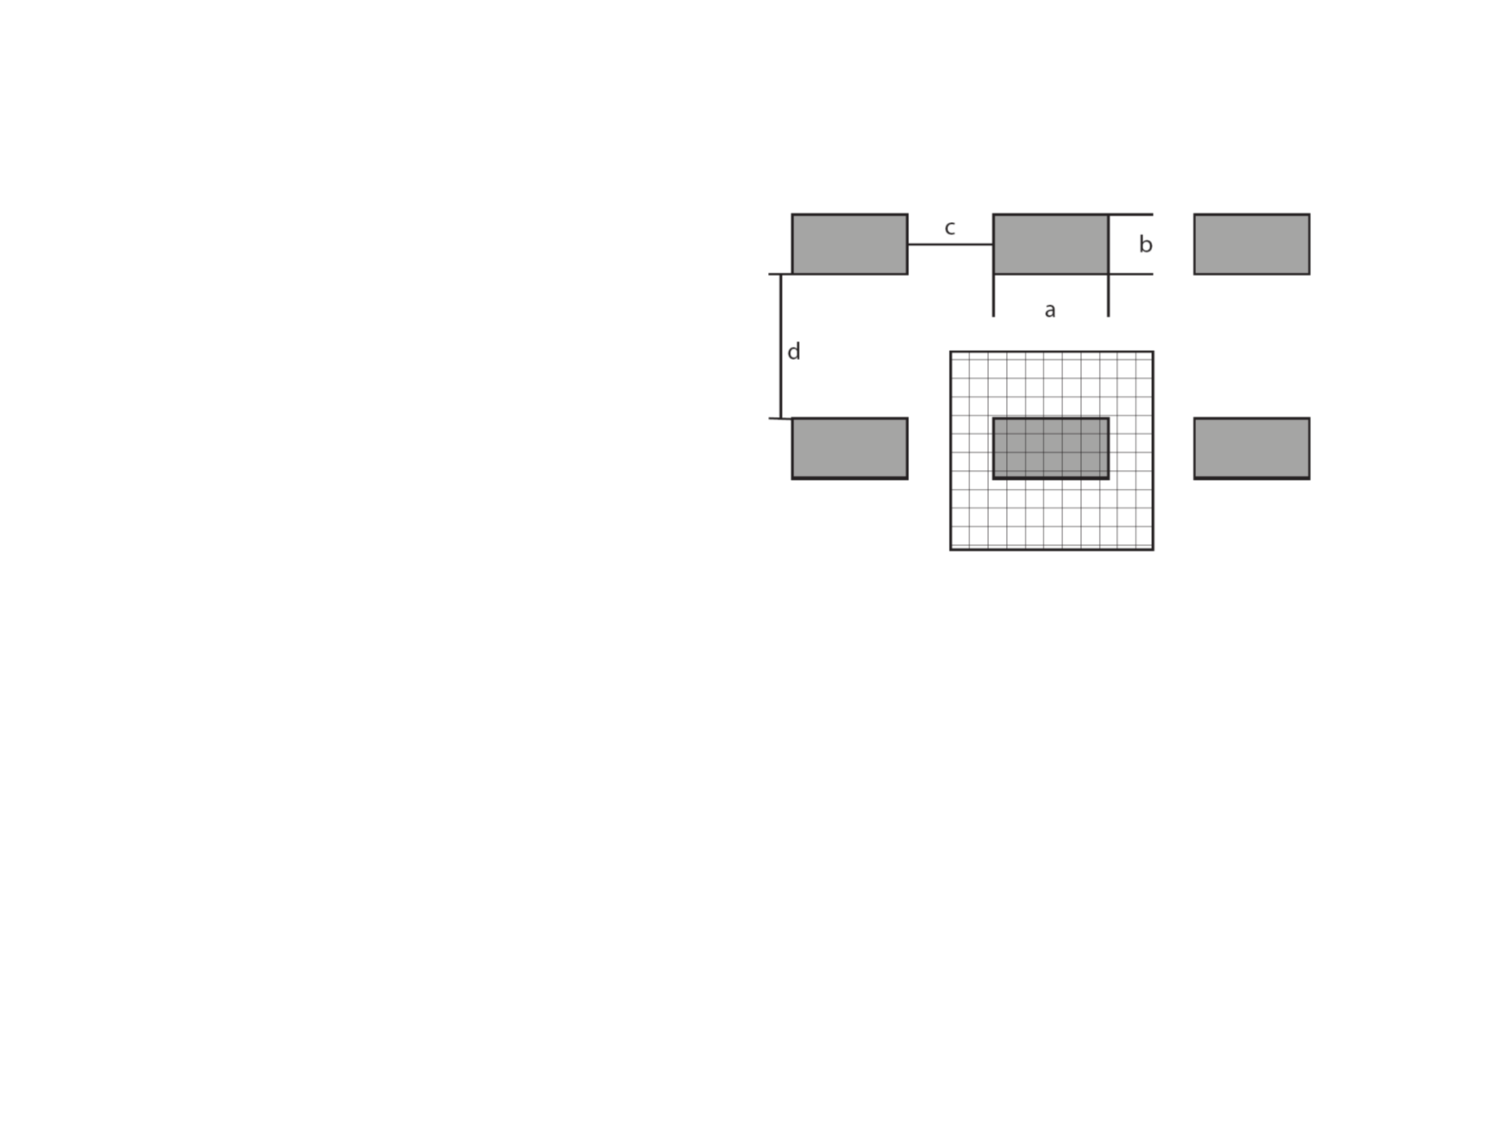
\includegraphics[width=0.8\textwidth]{Grafiken/Abbauverlust3d.pdf}
\end{minipage}



\subsection{Theoriefragen}

\begin{itemize}
    \item Geklüfteter Gestein - Bei einer hydraulischen Stimulation wurden maximale hydraulische Drücke gemessen, die kleiner als die in-situ Spannungen sind. Ist dieses Ergebnis zu erwarten?\\
    $\blacktriangleright$ Ja, die existierenden Klüfte werden aktiviert.
    
    \item Faktoren des Gebirgsaufbaus:\\
        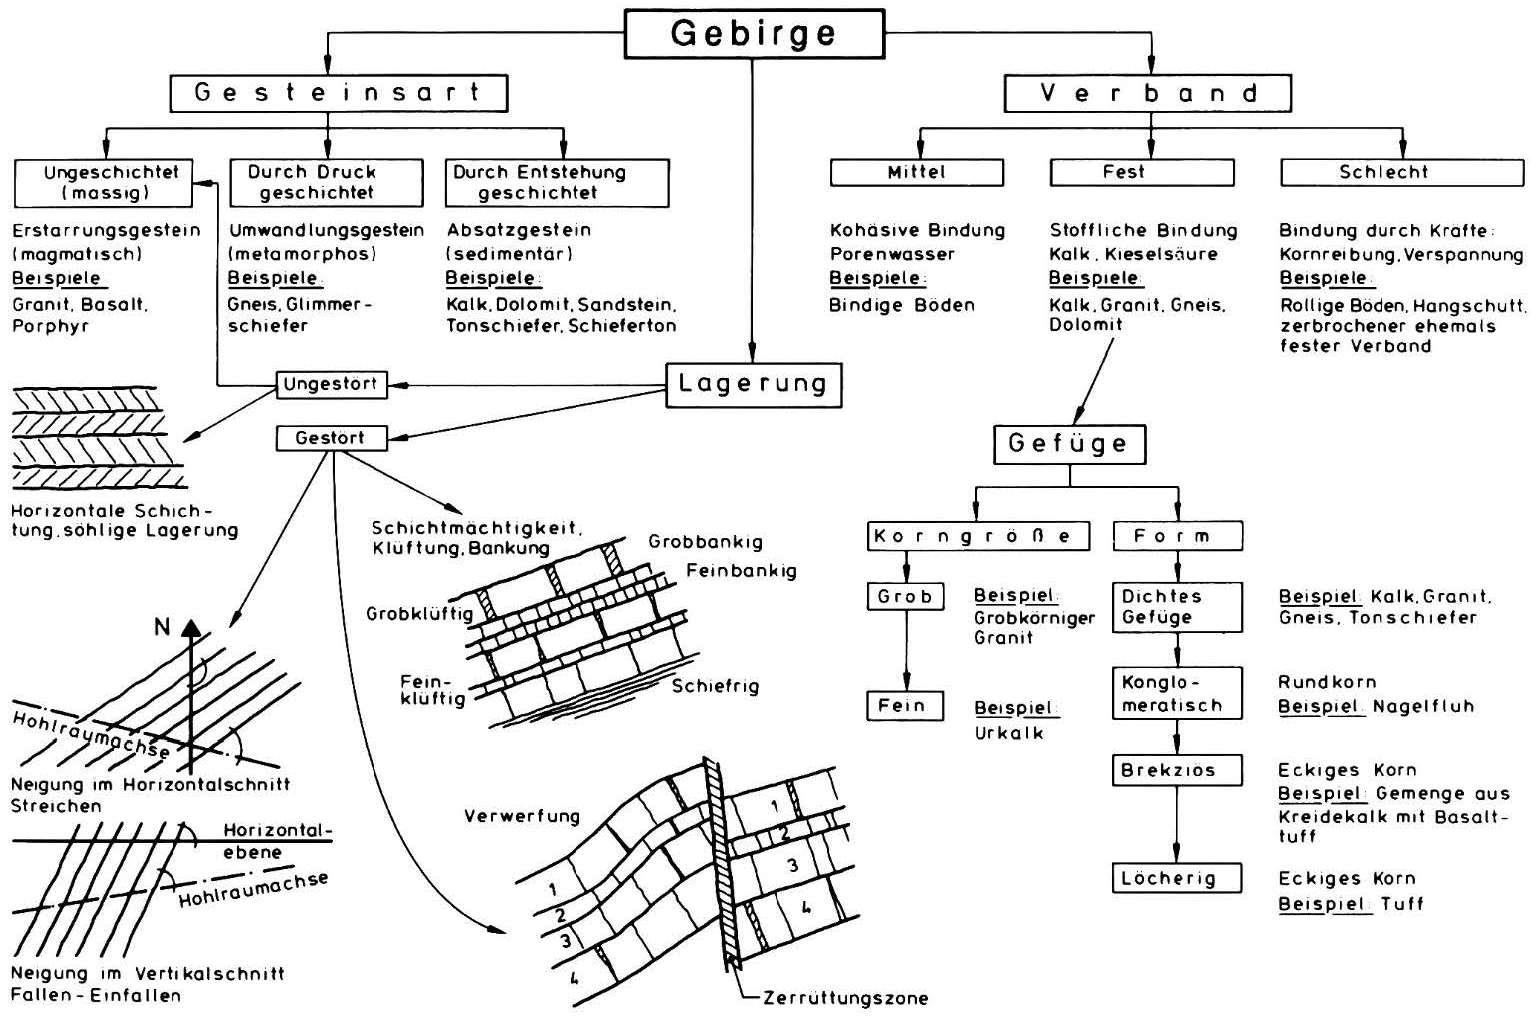
\includegraphics[width=0.8\textwidth]{Grafiken/Faktoren_Gebirgsaufbau.png}
\end{itemize}



%%%%%%%%%%%%%%%%%%%%%%%%%%%%%%%%%%%%%
%%%%%%%%%%%%%%%%%%%%%%%%%%%%%%%%%%%%%
%%%%%%%%%%%%%%%%%%%%%%%%%%%%%%%%%%%%%
%%%%%%%%%%%%%%%%%%%%%%%%%%%%%%%%%%%%%
%%%%%%%%%%%%%%%%%%%%%%%%%%%%%%%%%%%%%
%%%%%%%%%%%%%%%%%%%%%%%%%%%%%%%%%%%%%
%%%%%%%%%%%%%%%%%%%%%%%%%%%%%%%%%%%%%
%%%%%%%%%%%%%%%%%%%%%%%%%%%%%%%%%%%%%
%%%%%%%%%%%%%%%%%%%%%%%%%%%%%%%%%%%%%

%\newpage
\section{Tunnelbau}

\subsection{Aufbau Tunnel}
\begin{minipage}{0.6\textwidth}
    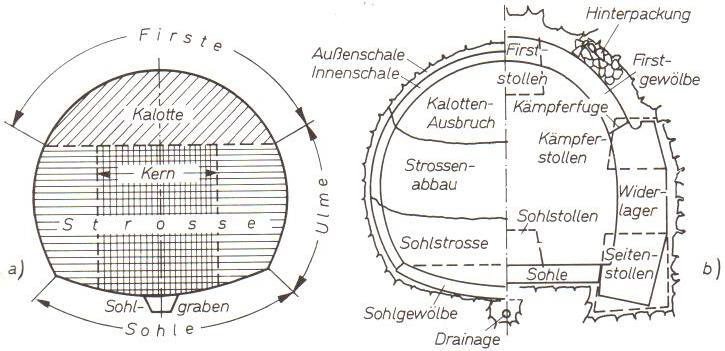
\includegraphics[width=0.99\textwidth]{Grafiken/Tunnel_Aufbau_1.png}
\end{minipage}
\begin{minipage}{0.3\textwidth}
    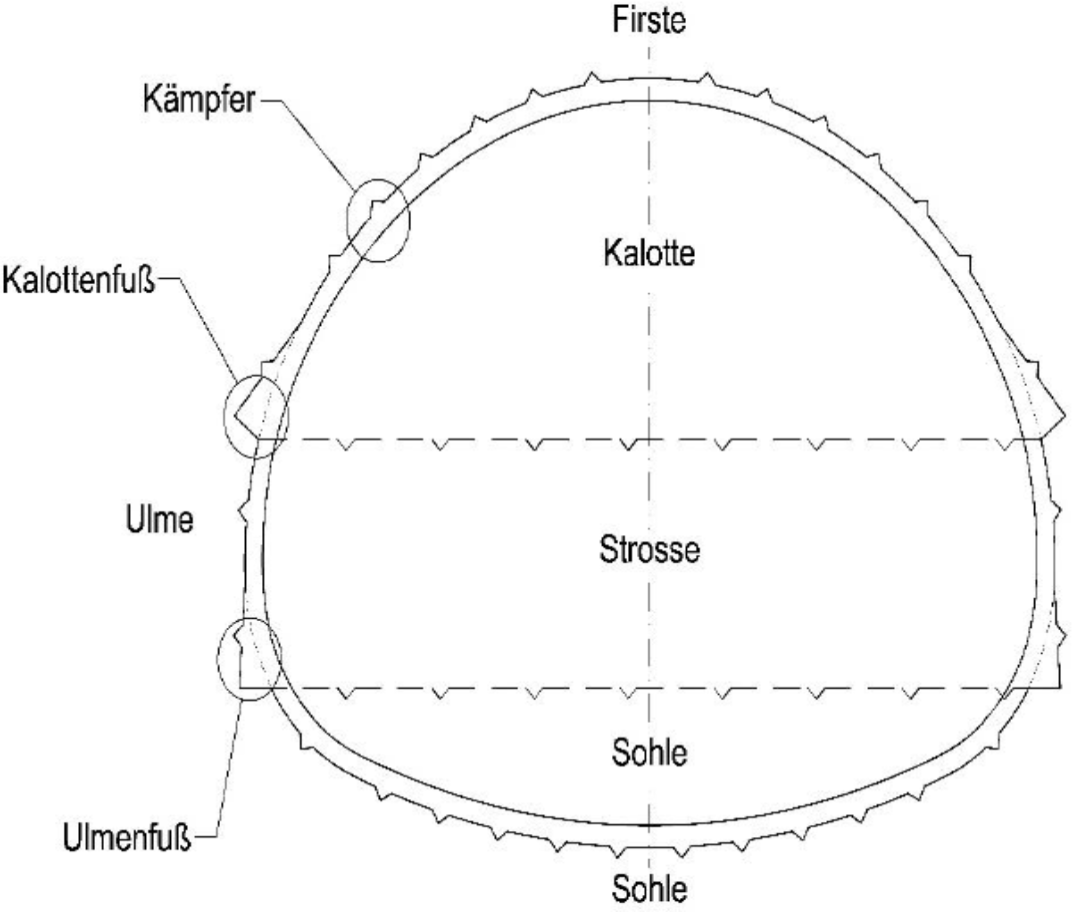
\includegraphics[width=0.99\textwidth]{Grafiken/Tunnel_Aufbau_2.png}
\end{minipage}



\subsection{Theoretische Grundlagen}
\begin{itemize}
    \item Grenze Einsatz von Teilschnittmaschinen: $F_{schi} \leq 0,5 \frac{N}{mm}$
        \begin{itemize}
            \item $F_{schi}=Q^{ast} \cdot \sigma_t \cdot d_{50}$
            \item $Q^{ast}=1,0 \cdot M_Q + 0,33 \cdot M_{Fsp} + 0,33 \cdot M_{Amph} + 0,33 \cdot M_{Px}$
        \end{itemize}
    \item Unterscheidung Stollen und Tunnel $\Rightarrow$ Stollen < 30$m^2$ ; Tunnel < 300$m^2$
    \item Einflussbereich Tunnel: $r_e = e \approx 6r_i=3d$
    \begin{itemize}
        \item Erklärung: In einem Abstand von 3 Tunneldurchmessern von der Tunnelwand ist der Einfluss der Spannungsänderung $\Delta\sigma$ durch den Tunnelausbau kleiner als 3\% und nicht mehr messbar.
    \end{itemize}
    \item Maßgebende Richtlinien:
        \begin{itemize}
            \item Deutsche Bahn: RiL 853
            \item Bundesstraßenbauverwaltung: ZTV-ING
        \end{itemize}
    \item Verdingungsordnung:
        \begin{itemize}
            \item Vortriebsklassen benannt: Verdingungsordnung für Bauleistung (VOB)
            \item Dort verwendete DIN-Norm: DIN 18312
        \end{itemize}
    \item Vortriebsklassen:
        \begin{itemize}
            \item \textbf{Vortriebsklasse 1:} Ausbruch ohne Sicherung.
            \item \textbf{Vortriebsklasse 2:} Ausbruch mit einer Sicherung, die in Abstimmung auf das Bauverfahren so eingebaut werden muss, dass das Lösen und Laden nicht behindert wird (Die Sicherung ist unabhängig vom Vortrieb).
            \item \textbf{Vortriebsklasse 3:} Ausbruch mit einer in definiertem Abstand zur Ortsbrust nachfolgenden Sicherung, für deren Einbau das Lösen und Laden unterbrochen werden muss (zyklischer Vortrieb).
            \item \textbf{Vortriebsklasse 4 und 4A:} Ausbruch mit unmittelbar folgender Sicherung. Bei der Vortriebsklasse 4 A ist zusätzlich eine Unterteilung des Ausbruchquerschnitts aus Gründen der Standsicherheit vorzunehmen.
            \item \textbf{Vortriebsklasse 5 und 5A:} Ausbruch mit unmittelbar folgender Sicherung einschließlich einer Sicherung der Ortsbrust. Bei der Vortriebsklasse 5 A ist zusätzlich eine Unterteilung des Ausbruchquerschnitts aus Gründen der Standsicherheit vorzunehmen
            \item \textbf{Vortriebsklasse 6 und 6A:} Ausbruch mit unmittelbar folgender und voreilender Sicherung. Bei der Vortriebsklasse 6 A ist zusätzlich eine Unterteilung des Ausbruchquerschnitts aus Gründen der Standsicherheit vorzunehmen.
            \item \textbf{Vortriebsklasse 7 und 7A:} Ausbruch mit unmittelbar folgender Sicherung einschließlich der Sicherung der Ortsbrust und voreilender Sicherung. Bei der Vortriebsklasse 7 A ist zusätzlich eine Unterteilung des Ausbruchquerschnitts aus Gründen der Standsicherheit vorzunehmen.
        \end{itemize}
\end{itemize}

\subsection{Sicherung und Ausbau} 
\begin{itemize}
    \item Stützmittelzahl: $S=\frac{A_L\cdot D}{ESR}$ oder $S=\frac{A_L\cdot H}{ESR}$ $_{\text{(März 2018 - 2)}}$
    \begin{itemize}
        \item $A_L$: Abschlagslänge
        \item $D$: Hohlraumdurchmesser
        \item $H$: Querschnittshöhe
        \item $ESR$: Ausbruch-Stützmittel-Faktor
    \end{itemize}
    \begin{table}[H]
    \hspace*{0.7cm}
        \begin{tabular}{|c p{13.3cm}|c|}
            \hline
             & \textbf{Ausbruchkategorie} & \textbf{ESR} \\ \hline
            A & temporäre Ausbrüche & 3-5 \\ \hline
            B & Schächte mit rundem Querschnitt & 2,5 \\ \hline
             & Schächte mit rechteckigem Queschnitt & 2,0 \\ \hline
            C & \begin{tabular}[c]{@{}l@{}}permanente Ausbrüche, nichtdruckhafte Wasserstollen für Wasserkraftanlagen, \\ Pilotstollen, Stollen und Richtstollen für große Ausbrüche\end{tabular} & 1,6 \\ \hline
            D & \begin{tabular}[c]{@{}l@{}}Lagerkavernen, Wasseraufbereitungsanlagen, kleinere Straßen- und Eisenbahntunnel, \\ Wasserschlösser und Zugangsstollen\end{tabular} & 1,3 \\ \hline
            E & \begin{tabular}[c]{@{}l@{}}Kraftwerke, große Autobahn- und Eisenbahntunnel, zivile Schutzbunker, \\ Portalbereiche, Verbindung von Tuunneln\end{tabular} & 1,0 \\ \hline
            F & unterirdische Atomkraftwerke, Eisenbahnstationen, Fabriken & 0,8 \\ \hline
        \end{tabular}
    \end{table}
    \item Erforderliche Ankerlänge: $L=\frac{2+0,15B}{ESR}$
    \begin{itemize}
        \item $B$: Tunneldurchmesser
    \end{itemize}
    \item Maximale ungesicherte Abschlagslänge: $A_{L,u}=2\cdot ESR \cdot \sqrt[5]{Q^2}$
    \item Permanenter Ausbaudruck: $ \left[ \frac{kg}{cm^2} \right] =\frac{2}{J_r}\frac{1}{\sqrt[3]{Q}}$
    \begin{itemize}
        \item $Q$ und $J_r$ aus \autoref{Q}
    \end{itemize}
    \item Ankerabstand in Querrichtung: $a=\frac{(L-d_{geb,1})\cdot2r_0\cdot \tan(\kappa)}{d_{geb,1}+r_0}$
    \item Ankerabstand in Längsrichtung: $b=\frac{a(r_0+L)\cdot2\tan(\kappa)}{2r_0\tan(\kappa)+a}$
    \begin{itemize}
        \item Dicke Gebirgstragring in Querrichtung: $d_{geb,1}=L-\frac{a(r_0+L)}{2r_0\tan(\kappa)+a}$
        \item Dicke Gebirgstragring in Längsrichtung: $d_{geb,2}=L-\frac b{2\tan(\kappa)}$
        \item $r_0$: Radius des freien Querschnitts
        \item $L$: Länge der Anker
        \item $\kappa$: Krafteinleitungswinkel i.d.R. $45^\circ$
    \end{itemize}
\end{itemize}

\subsection{Tagbruch - treibende und haltende Kräfte}
\begin{itemize}
    \item Treibende Kraft: $G = \gamma \cdot l_{\text{Längsrichtung}} \cdot h_{\text{Überlagerung}} \cdot b_{\text{Kalotte}}$\\
    Höhe 2 Möglichkeiten: Nur $h_1$=überlagerung oder $h_2$=Überlagerung+(Tunnelhöhe-Tunnelvortriebshöhe)
    \item Haltende Kraft aus Reibung: $R = n_{Seiten} \cdot (0,5 \cdot \gamma \cdot h^2 \cdot \tan(\varphi))$\\
                            mit Seitendruckumlagerung: $R = n_{Seiten} \cdot (0,5 \cdot \gamma \cdot h^2 \cdot \lambda (\text{oder}\, \nu)\tan(\varphi))$
    \item Haltende Kraft aus Kohäsion: $C = n_{Seiten} \cdot (c_u \cdot h)$
    \item Anker nötig: $F_{Anker} = G - R - C$
    \item Grundbruchbetrachtung Kalottenfüße: $\eta = \frac{R+C+N_{Fund}}{G} \overset{!}{\geq} 1$
    \item $N_{Fund} =$ Grundbruchnachweis
    \item Sicherheit der Spritzbetonschale gegen Durchscheren. Kritische Breite = 0,707b. Scherung unter 45$\circ$.\\
            $S_{Spritzbeton}=2 \cdot 1,414 \cdot d_{Spritzbet.} \cdot \tau_{Beton} \cdot \sigma_{u,Beton}$
\end{itemize}

%\newpage
\subsection{Theoriefragen}
\begin{small}
\begin{itemize}
    \item Tunnelradius zu Bettung: \enquote{Je kleiner der Radius, desto größer die Bettung}: $k = \frac{E}{r}$
    \item Drucker-Prager Verfahren: Man kann rechnerisch mehr aus dem Material holen.
    \item \textbf{Vorentlastungsfaktor $\alpha$} zur Berücksichtigung \textbf{räumliche Tragwirkung}
        \begin{itemize}
            \item reduzierte Steigkeit: $E_{red} = \alpha \cdot E$
            \item Gebirgsverhältnisse:
                \begin{itemize}
                    \item $\alpha$ kann nahe an 1 oder 0 gewählt werden, z.B. $\alpha = 0,9$: Gebirge mit geringeren Festigkeiten, damit geringere Vorentlastung, aber geringere Verformung und höhere Belastung des Ausbaus; $\alpha = 0,1$: Gebirge mit großer Festigkeiten, damit größere Vorentlastung, aber größere Verformung und geringere Belastung des Ausbaus.
                \end{itemize}
        \end{itemize}
    \item \textbf{Nichtlineare Materialmodelllierung Berechnungsverfahren:}\\
    $\blacktriangleright$ Iterative Berechnung der Spannungs/Verformungszustände, dabei wird so lange programmintern variiert bis ein Gleichgewichtszustand erreicht ist.
    \item \textbf{Verwendbare Festigkeitskriterien:}\\
    $\blacktriangleright$ Mohr-Coulomb, Drucker-Prager
    \item \textbf{Sicherungsmittel zur Ortsbruststützung}:\\
    $\blacktriangleright$ Bewehrter Spritzbeton, Nägel/Anker, Brustkeil/Stützkern, Unterteilung der Ortsbrust/Ulmenstollenvortrieb
    \item Was besagt das \textbf{Kennlinienverfahren im Tunnelbau} bezüglich des \textbf{Zusammenwirkens von Gebirge und Ausbau}? Erläutern an einer Kennlinie für Gebirge mit elastoplastischem Verhalten inkl. Entfestigung in Kombination mit einer Spritzbetonschale\\
    $\blacktriangleright$ Kennlinie eines Gebirges gibt erforderlichen Ausbauwiderstand (Ordinate) über die Zeit/Gebirgsverschiebung (abszisse) an. Zunächst fällt (schematisch) die Kurve linear ab, dann nehmen die Verschiebungen bei der weiteren Reduzierung der Gebirgsstützung überproportional zu. Wenn man die Auflockerung und Entfestigung des Gebirges dann weiter zulässt, nimmt der erforderliche Ausbauwiderstand sogar wieder zu. Der Ausbau ist also früh und so stark einzubauen, dass die Kennlinie des Ausbaus die Kennlinie des Gebirges schneidet, bevor das Minimum des erforderlichen Ausbauwiderstands überschritten wird. In der Regel ist der Ausbau sehr früh und tragend einzubauen, da der Spritzbeton seine Steifigkeit entwickeln muss. Dass heißt: Die Kennlinie des Spritzbetons beginnt auf der Abszisse nicht im Ursprung, die Neigung seiner Kennlinie wird mit zunehmender Zeit steiler, weil der E-Modul mit der Zeit zunimmt und somit der Widerstand gegen die Gebirgsverschiebung.
    \item Was besagt das Kennlinienverfahren im Tunnelbau bezüglich des Zusammenwirkens von Gebirge und Ausbau? Erläutern Sie das Verfahren an einer Kennlinie für Gebirge mit elastoplastischem Verhalten inkl. Entfestigung in Kombination mit einer SpritzbetonauBenschale\\
    $\blacktriangleright$ Die Kennlinie des Gebirges gibt den erforderlichen Ausbauwiderstand (Ordinate) über die Zeit/Gebirgsverschiebung (Abszisse) an. Zunächst fällt (schematisch) die Kurve linear ab; dann nehmen die Verschiebungen bei der weiteren Reduzierung der Gebirgsstützung überproportional zu. Wenn man die Auflockerung und Entfestigung des Gebirges dann weiter zulässt, nimmt der erforderliche Ausbauwiderstand sogar wieder zu. Der Ausbau ist also so früh und so stark einzubauen, dass die Kennlinie des Ausbaus die Kennlinie des Gebirges schneidet, bevor das Minimum des erforderlichen Ausbauwiderstands überschritten wird. In der Regel ist der Ausbau sehr früh und tragend einzubauen, da der Spritzbeton seine Steifigkeit entwickeln muss. D. H.: Die Kennlinie des Spritzbetons beginnt auf der Abszisse nicht im Ursprung; die Neigung seiner Kennlinie wird mit zunehmende Zeit steiler, weil der E-Modul mit der Zeit zunimmt und somit der Widerstand gegen die Gebirgsverschiebungen. Nur für den Fall von sehr tiefliegende Tunnel - bzw. bei einer relativ geringen Gebirgstragfähigkeit und geringer Gebirgssteifigkeit im Verhälthis zum Gebirgsdruck führen die Zwängungen infolge Gebirgsdeformation zu so hohen Spannungen im Ausbau, dass die Spritzbetonschale zerstört wird. In diesem Fall lässt man in der Spritzbetonschale zunächst Deformationsschlitze (ggf. mit nachgiebigen Druckelementen aus hydraulischen Zylindern), die man erst nach der ersten Gebirgsberuhigung dann mit Beton einspritzt. Die Bewehrung ist dann vollständig auch in den Deformationsschlitzen versiegelt. In besonderer Weise ist die Tunnelschale aus Spritzbeton bei der Ausführung mit den Deformationsschlitzen mit Ankern zu sichern, damit man ein duktiles System aus Ankern, Spritzbeton und Gebirge erhält.
    \item Erklären sie die \textbf{Wirkungsweise der Gebirgsankerung einer Spritzbetonschale}.\\
    $\blacktriangleright$ Die Wirkung beruht auf vier Gesichtpunkten:
    \begin{enumerate}
        \item Im $\tau - \sigma$-Diagramm wird die Tangentialspannung als größte Spannung $\sigma_1$ und der Ausbauwiderstand als kleinste Spannung $\sigma_3$ dargestellt. Die Ankerung erhöht den Innendruck, so dass eine höhere Tangentialspannung aufgenommen werden kann. Der Ausbauwiderstand infolge der Ankerung ist allerdings so gering, dass die positive Wirkung der Anker dadurch nicht quantitativ erklärt werden kann.
        \item Die Ankerung erhöht die Scherfestigkeit des Gebirges. Dies wird in Berechnungen berücksichtigt durch eine höhere Kohäsion.
        \item Analog der Endflächenreibung in einachsialen Druckversuchen - bei denen die Festigkeiten umso größer werden umso geringer das Verhältnis der Höhe zum Durchmesser der Prüfkörper wird - kann man den belasteten Gebirgsbereich als Bereich zwischen den Ankern betrachten. Je länger die Anker sind und je geringer der Ankerabstand ist, umso besser ist die Tragfähigkeit. Die Anker erfüllen die Wirkung der Endflächenreibung im einachsialen Druckversuch. Rechnerisch ergeben sich aber Ankerquerschnitte, die dicker als die üblich verwendeten Ankerquerschnitte sind. Die Gebirgsfestigkeit wird erhöht.
        \item Durch die Ankerung des Gebirges wird die Gebirgsentfestigung im post-failure Bereich einer $\sigma - \epsilon$-Kurve verhindert. Es kommt nicht so sehr auf eine sehr hohe Gebirgsfestigkeit an, die ein elastisches Gebirge darstellt; vielmehr ist wird durch die Anker die Entfestigung des Gebirges vermieden bzw. reduziert und eine Mindestfestigkeit des Gebirges gewährleistet.
    \end{enumerate}    
    \item In welchen Fällen wird eine \textbf{zusätzliche Tunnelinnenschale} eingebaut, obwohl der Tunnel mit der Außenschale nach der Auffahrung standsicher ist. Gegen \textbf{welche Einwirkungen} benötigt man die Tunnelinnenschale?\\
    $\blacktriangleright$ Die Tunnelinnenschale ist auf Grund folgender Gründe erforderlich:
    \begin{enumerate}
        \item Das Bergwasser ist aggressiv und die Außenschale wird angegriffen.
        \item Der Tunnel soll einen tropfwasserfreien und eisfreien Fahrweg haben; dazu reicht ein dichtes Innenschalengewölbe aus.
        \item Der Tunnel soll abgedichtet werden, damit auf Dauer der Bergwasserspiegel wieder ansteigt und der Tunnel nicht als Dränage wirkt.
        \item Spätere Einwirkungen wie Quelldrücke infolge quellfähigen Tonmineralen und/oder Anhydrit sind zu erwarten, die die Außenschale noch nicht belasten.
    \end{enumerate}
    \item Bei einem Tunnelvortrieb werden im Kalottenvortrieb \textbf{relativ große vertikale Verschiebungen der Firste} und \textbf{in ähnlicher Größe an den Kalottenfüßen} gemessen.
    \begin{enumerate}
        \item Wie erklären Sie dieses Verhalten, wenn der \textbf{horizontale Abstand} zwischen den Ulmenfüßen \textbf{nahezu konstant} bleibt?\\
        $\blacktriangleright$Wenn die Kalottenfußsetzungen ähnlich groß wie die Firstsetzungen sind, muss vermutet werden, dass die Kalottenfüße nicht technisch einwandfrei gegründet sind. Es besteht die Möglichkeit, dass eine sehr weiche oder aufgelockerte Schicht im Bereich der Kalottenfüße ansteht oder dass ausgebrochenes Gebirge nicht komplett im Fußbereich ausgeräumt wurde. Aus der Beobachtung, dass keine Konvergenzen auftreten, ist eine geringe horizontale Belastung zu vermuten, da die vertikale Belastung nicht sehr groß sein kann, wenn die Kalottenfüße nachgeben. Aus der Beobachtung, dass keine Divergenzen auftreten und sich die Kalottenfüße ähnlich wie die Firste setzen, kann gefolgert werden, dass die vertikale Belastung der Kalotte noch gering ist.
        \item Wie beurteilen Sie die Ausnutzung der Tragfähigkeit des Kalottengewölbes?\\
        $\blacktriangleright$Aus der Translation des Kalottengewölbes ergibt sich, dass die Spritzbetonschale keine Biegebeanspruchung erfährt und die Ausnutzung der Tragfähigkeit noch sehr gering ist.
        \item  Welche Maßnahmen empfehlen Sie im Tunnelvortrieb zur Verbesserung des Tragverhaltens und Verringerung der Verschiebungen?\\
        $\blacktriangleright$ Zwei Aspekte sind zu beachten, um die Kalottenfußsetzung zu reduzieren:
        \begin{enumerate}
            \item Die Bauüberwachung und die Bauleitung müssen durch Kontrolle ausschließen, dass aufgelockertes, ausgebrochenes Gebirge im Bereich der Kalottenfüße verbleibt.
            \item Im Falle einer natürlich anstehenden, weichen Schicht unter den Kalottenfüßen ist planerisch zu überprüfen, ob die Kalottenfußsetzungen verringert werden können:
            \begin{itemize}
                \item durch Ausräumung einer gering mächtigen weichen Schicht unter dem Kalottenfuß oder
                \item durch eine Kalottenfußverbreiterung oder
                \item durch \enquote{Pfähle} unter den Kalottenfüßen (wenn der Abschnitt mit diesem Setzungsverhalten sehr begrenzt erwartet wird) oder
                \item ob der Einbau eines Sohlgewölbes erforderlich ist (vorausgesetzt, der Fall "Ausbruchmaterial unter den Füßen" ist ausgeschlossen).
            \end{itemize}
            \end{enumerate}
    \end{enumerate}
    
    \item Welche \textbf{Sicherungsmittel und Ausbauabfolge für die Außenschale} schlagen Sie bei der Auffahrung eines zweispurigen Straßentunnels in \textbf{sehr druckhaftem Gebirge} mit \textbf{großen Verformungen} und \textbf{großer Überlagerungshöhe} vor?\\
    $\blacktriangleright$ Da das Gebirge sehr druckhaft ist und der Ausbruch zu großen Gebirgsverformungen führt, müssen die Sicherungsmittel
        \begin{itemize}
            \item sehr früh eingebaut werden und
            \item sehr flexibel sein.
        \end{itemize}
    Der frühe Einbau der Sicherung soll die Deformationen und die damit einhergehende Gebirgsentfestigung begrenzen. Als Sicherungsmittel kommen lange, schlaffe, voll vermörtelte Anker mit einer hohen Ankerungsdichte (Anker je m² Abwicklungsfläche) infrage. Dadurch wird ein geankerter Gebirgstragring erzeugt, der sich als armiertes Gebirge weniger stark entfestigt und ein großes Arbeitsvermögen hat. Als Ankertyp können GEWI Felsnägel oder Selbstbohranker verwendet werden, besonders wenn die Klüfte des Gebirges die Zementverpressung aufnehmen können; unter manchen Randbedingungen sind auch Swellex-Anker sinnvoll. Da die Ankerköpfe das Gebirge auf der Ausbruchseite nicht flächenhaft stützen, ist zusätzlich eine flexible Spritzbetonsicherung erforderlich. Die Flexibilität wird erhalten durch eine dünne, aber mit Baustahlmatten bewehrte Spritzbetonschicht, die mehrere über den Umfang verteilte Dehnungsschlitze enthält. Die Dehnungsschlitze werden derart ausgebildet, dass in ihnen ein flexibler, sich überlappender Bewehrungsstoß ohne Spritzbeton hergestellt wird. Nach dem Abklingen der Gebirgsverschiebungen wird die Spritzbetonschale verstärkt und die Dehnungsschlitze mit Spritzbeton verschlossen. Eine bessere, aber deutlich aufwendigere Variante für den nachgiebigen Spritzbetonausbau erzielt man durch den Einbau von Druckzylindern in die Dehnungsschlitze. Dann bewirkt die Spritzbetonschale einen zusät Ausbauwiderstand. Sie wird aber nicht durch zu große Gebirgsbelastungen und Zwängungen zerdrückt, weil unter hohen Betondrücken in Umfangsrichtung die hydraulischen Zylinder nachgeben. In beiden Fällen bleibt mit Ankern armierte Gebirge das wesentliche Tragelement mit großem Arbeitsvermögen und reduziertem Festigkeitsabfall im post failure Bereich der Spannungsdehnungslinie des Gebirge; ohne Ankerung wäre der Festigkeitsabfall sehr groß.
    
    \item Situation: Ein alter Eisenbahntunnel ohne Sohlgewölbe, der für zweigleisigen Betrieb gebaut wurde, aber nur eingleisig genutzt wird, zeigt \textbf{Ausbauschäden im Ziegelsteinmauerwerk, Nassstellen und Deformationen}. In Tunnelmitte liegt ein Längskanal zur Wasserableitung. Der ungestörte Grundwasserspiegel lag vor dem Bau des Tunnels deutlich über der Firste; der Tunnel senkt das Grundwasser im Gebirge über die durchlässige Gesteinshinterpackung (zwischen Ausbau und Gebirge) auf das Niveau der Dränagen im Tunnel ab. Der Platzbedarf im Tunnel ist jedoch nicht ausreichend, um eine allein tragende neue Ortbetoninnenschale einzubauen, so dass zur Erhöhung der Standsicherheit bautechnisch eine zusätzliche, rückverankerte Spritzbetonschale vorgesehen ist. Das Gebirge besteht aus einer Wechsellagerung aus Ton- und Sandstein. Die Schichtung fällt ca. 25° quer zum Tunnel ein. Das Gestein ist bereichsweise deutlich entfestigt und teils klüftig, überwiegend stark klüftig, bereichsweise jedoch sehr stark klüftig. Die Tonsteine sind dünnplattig und die Sandsteine überwiegend dickplattig ausgebildet. Die Überlagerungshöhe beträgt bis zu 50 m und der Tunnel ist 300 m lang.
    \item Welche \textbf{Erkundungsmaßnahmen} schlagen Sie für die \textbf{Beurteilung der IST-Standsicherheit} vor?\\
    $\blacktriangleright$ Bei einem bestehenden alten Tunnel ist weder die Tragfähigkeit noch die Belastung des Mauerwerksgewölbes bekannt. I. d. R. liegen über das Gebirge keine quantitativ verwertbaren Angaben zum festigkeitsmechanischen Verhalten vor. Deshalb sind der Ausbau und das Gebirge zu untersuchen:\\
    Ausbauuntersuchung:
    \begin{itemize}
        \item Ausbaudicke, Gesteins- und Mörteldruckfestigkeit an Standardbohrkernmaterial (Ø 100 mm) oder Mauerwerksfestigkeit an großen Bohrkernen (Ø 500 mm radial, aus den ca. Ø 300 mm Bohrkerne in Umfangsrichtung entnommen werden.)
        \item Ermittlung der Gründungstiefe und -breite der Widerlager
        \item Spannungsmessungen im Mauerwerk nach der Kompensationsmethode an der Innenrandfaser an mehreren Stellen des Umfangs; auf dieser Basis können dann Rückrechnungen zur Ermittlung der Verteilung der Gebirgsdrücke auf den Ausbau durchgeführt werden.
        \item Bestimmung der Abschalungen im Ausbaumauerwerk
        \item Erkundung, ob die Dränageleitungen in Ordnung sind
        \item Untersuchung der Schotterstärken auf dem Planum unter den Schwellen
        \item Erkundung der Dicke der Hinterpackung zwischen Ausbau und Gebirge in den Ulmen und in der Kalotte ggf. ergänzend mit geophysikalischen Methoden
        \item Chemische Untersuchung der Abdichtung (meist nur auf dem Kalottengewölbe vorhanden)
    \end{itemize}
    Gebirgsuntersuchungen:
    \begin{itemize}
        \item Erkundung des geologischen Aufbaus an Hand von Geologischen Karten, Literatur
        \item Dokumentation des Gebirges in den Voreinschnitten, in den Sicherheitsnischen im Tunnel und in natürlichen und künstlichen Aufschlüssen der Umgebung
        \item Bestimmung der festigkeitsmechanischen Eigenschaften
        \item Untersuchung der Grundwasserbeschaffenheit, insbes. bzgl. Beton und Stahlaggressivität.
        \item Dokumentation, welche Wassermengen die Dränagen abführen.
        \item geotechnische Laborversuche zur Standsicherheit und Lösbarkeit des Gebirges (Abrasivität)
        \item Mineralogische Untersuchungen, chemische Untersuchungen, auch hinsichtlich der Entsorgung von Ausbruchmaterial.
        \item Bestimmung des Quellpotentials der Tonsteine
        \item Scherfestigkeit der Anisotropieflächen, insbesondere der tonigen Schichtflächen
    \end{itemize}
    \item Beschreiben und begründen Sie Ihre \textbf{Wahl der Ankersicherung hinsichtlich des Gebirges, der Hinterpackung und der Dränagewirkung} des bestehenden Tunnels.\\
    $\blacktriangleright$ Da davon auszugehen ist, dass zwischen dem Ausbau und Gebirge eine Gesteinshinterpackung eingebaut ist. Weiterhin ist das Gebirge infolge der Schichtung und Klüftung in den Bohrungen nicht allgemein standsicher, so dass kleine Steine in das Bohrloch nachbrechen. (Schichtdicke und Kluftabstände: überwiegend 5 - 10 cm, bereichsweise 1 - 5 cm). Demzufolge ist es schwierig, bei Verwendung von GEWI Felsnägeln nach der Herstellung des Bohrlochs dieses mit einem Mörtelschlauch hinter der Hinterpackung zu treffen bzw. das Bohrloch ist nicht mehr durchgängig offen in der Hinterpackung und im anstehenden Gebirge. Deshalb scheidet der Einbau von GEWI Felsnägel aus und es werden stattdessen Injektionsbohranker / Selbstbohranker verwendet. Bei diesen Ankertypen verbleibt das Bohrgestänge mit einer verlorenen Bohrkrone als Anker im Bohrloch. Die Mörtelverfüllung erfolgt über das im Bohrloch verbliebene Bohrgestänge vom Bohrlochtiefsten aus. Die Mörtelmenge ist zu begrenzen auf z. B. das 2 bis 3 fache des Bohrlochvolumens, damit die Dränagewirkung der Hinterpackung erhalten bleibt. Daraus folgt aber auch, dass der Anker im Bereich der Hinterpackung und des Mauerwerks keine vollständige Zementsteinüberdeckung hat, die den Korrosionsschutz gewährleistet. Deshalb ist der Stahlquerschnitt dicker auszuführen als statisch erforderlich, um so eine Abrostrate einer z. B. 2 mm dicken Opferschicht vorzuhalten; die Abrostungsdicke ist entsprechend der angestrebten Lebensdauer und dem Wasserchemismus unterschiedlich dick zu wählen. Wenn im Bereich der Mauerwerksbohrung keine Zementsteinummantelung gegeben ist, sollte ggf. dieses Bohrloch nachverpresst werden.
    Als Bohrlochverfüllung ist ein Wasser-Zement-Gemisch ungeeignet. Es ist ein thixotroper Ankermörtel zu verwenden, der auch in Bohrlöchern nach oben nicht aus dem Bohrloch heraus rinnt. Die Länge der Anker ist in Relation zu der Ankerdichte so zu wählen, dass ein ausreichend dicker, armierter Gebirgstragring mit dem bestehenden Mauerwerksgewölbe erzeugt wird. Wenn möglich, sind die Anker bis in das nicht aufgelockerte Gebirge zu setzen.Wird vor den Widerlagem z. B. wegen der Entwässerung die Einbindetiefe der Widerlager verhindert oder zeigen sich wegen des Schichteinfallens quer zum Tunnel Ulmende formationen, so ist der Widerlagerfuß gezielt durch eine Ankerung zu sichern. Die Widerlager sind hinsichtlich Grundbruch und Gleiten, besonders wegen der Horizontalkräfte statisch gezielt zu betrachten.
    \item Beschreiben und begründen Sie Ihre \textbf{Wahl der Ausführung der Spritzbetonsicherung}.\\
    $\blacktriangleright$ Die dünne, armierte Spritzbetonschale ist nicht allein tragendes Ausbauelement; er trägt vielmehr im Verbund mit dem weiter mitwirkenden Mauerwerksgewölbe. Der armierte Spritzbeton bildet somit die Zugfaser eines dicken, verstärkten Mauerwerks. Die Spritzbetonschale sollte mindestens ca. 15 cm dick gewählt werden, damit die Betondeckung von 6 cm beidseitig der einzulegenden Baustahlmatte gewährleistet ist. Sie ist zweilagig zu spritzen. Die Spritzbetonschale mit dem Mauerwerk mittels Dübel zu verbinden ($\geq$ 4 St./m²). Die Dübel müssen in das kompakte Mauerwerk einbinden, d. h. bei Ziegelsteinmauerwerk bis hinter die erste Läuferschicht (211 cm plus Einbindung = ca. 20 cm lang). Bei den Spritzbetonarbeiten ist darauf zu achten, dass der bestehende Gleisschotter und eine ggf. vorhandene Oberleitung nicht \enquote{verschmutzt} werden    
    \item Beschreiben und begründen Sie Ihre \textbf{Wahl für die Entwässerung im Endzustand}.\\
    $\blacktriangleright$ Das bestehende Mauerwerksgewölbe ist nicht auf Wasserdruck dimensioniert. Bei der durchlässigen Hinterpackung und der offenen Sohle ist der GW Spiegel zum Tunnel hin auf das Sohlniveau abgesenkt. Da der Tunnel als Gebirgsdränage rechtlich Bestandschutz hat, soll das GW auch weiter dauerhaft abgesenkt werden. Die Durchlässigkeit der Hinterpackung muss weiter gewährleistet werden. Nassstellen im Mauerwerk sollen nur in Ausnahmefällen durch Anbohren und Injektionen abgedichtet werden. Dass Wasser tritt ansonsten an anderen durchlässigen Mauerwerksbereichen aus. Es ist sinnvoll, die Nassstell gezielt anzubohren und eine Dränleitung auf dem Mauerwerk hinter dem Spritzbeton einzubauen. Die Dränage kann bestehen aus einem mit Vlies oder Kokosfasern ummantelten Schlauch, aus einem Streifen Noppenfolie oder aus einem Kammerdrän. Vor den Widerlagern ist das Bergwasser in eine Längsleitung einzuleiten. Die Längsleitung soll frostfrei eingebunden bzw. überschüttet werden. In regelmäßigen Abständen, z. B. 50 m, sind Revisions- und Spülschächte vorzusehen.
    
    \begin{minipage}{0.69\textwidth}
        \item Zeichnen sie qualitativ die \textbf{Kennlinie des Gebirges} und des \textbf{Ausbaus aus Spritzbeton} an der Firste.\\
        $\blacktriangleright$ Die Firste plastifiziert. Das bedeutet, dass die Verschiebung nicht eine lineare Funktion des Drucks ist. Entfestigung kann stattfinden oder nicht. $\frac13$ der Verschiebung hat schon an der Ortsbrust stattgefunden. Der Spritzbeton wird mit der Zeit steifer.
    \end{minipage}		
    \begin{minipage}{0.3\textwidth}
        $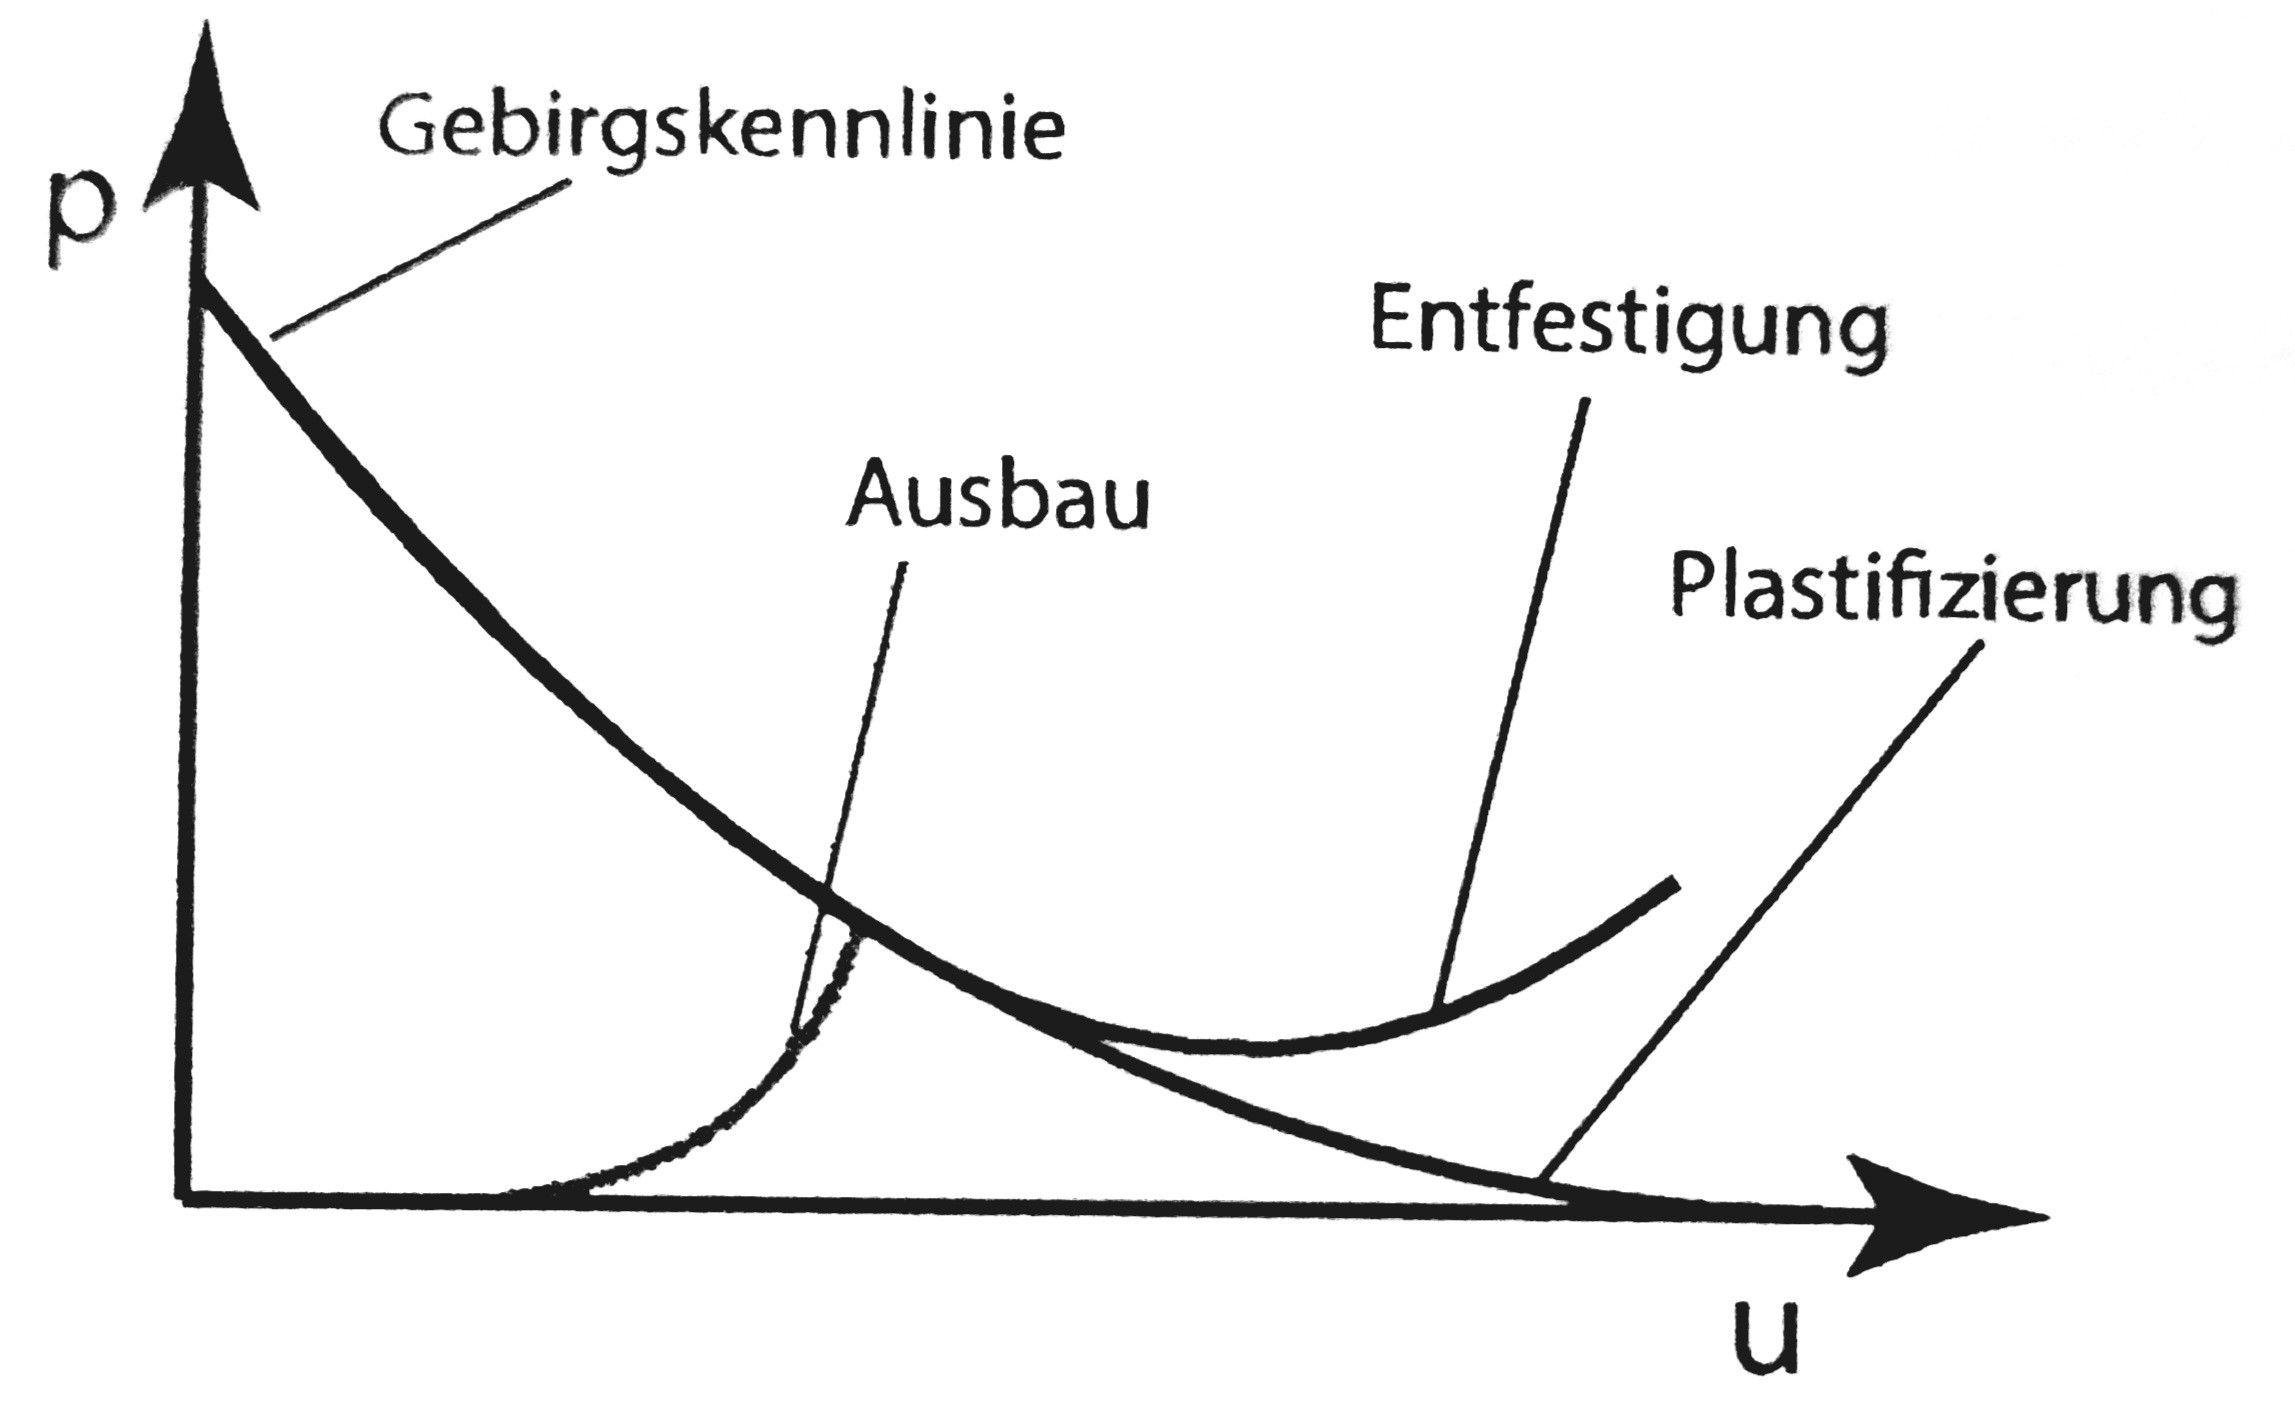
\includegraphics[width=0.8\textwidth]{Grafiken/Kennlinie_Ausbau_Gebirge.jpg}$
    \end{minipage}
    
    \item Welche \textbf{Folgerungen} hätte man \textbf{aus} den \textbf{Verschiebungsmessungen im Tunnel} ziehen müssen? (Gleichmäßige Setzung über gesamte Länge)\\
    $\blacktriangleright$ Aus der Beobachtung, dass sich die Kalottenfüße und die Firste annähernd in gleicher Größenordnung vertikal nach unten verschieben, muss gefolgert werden, dass die Tragfähigkeit der Kalottenfüße nicht ausreichend groß ist. Dies kann dadurch bedingt sein, dass die Kalottensohle unter den Kalottenfüßen nicht ausreichend beräumt wurde. Die Kalottenfußsetzungen können aber auch dadurch bedingt sein, dass das Gebirge unter den Kalottenfüßen keine ausreichende Tragfähigkeit hinsichtlich Grundbruch hat bzw. unter den Kalottenfüßen eine weiche, stark verformbare Tonsteinschicht liegt. Bei einer gleichmäßigen Verschiebung (Translation) der Kalotte ergeben sich zwar keine Biege spannungen in der Spritzbetonaußenschale, diese kann aber insgesamt kollabieren. Deshalb ist auch die messtechnische Überwachung in Querprofilen über dem Tunnel an der GOF erforderlich. Auf Grund der Größe der Setzungen ist davon auszugehen, dass sich das Gebirge nicht (mehr) dilatant verhält sondern schon infolge Auflockerung entfestigt ist. Das Ausbausystem Tonstein und Spritzbetonschale wirkt nicht ausreichend duktil, so dass entsprechende zusätzliche Sicherungen notwendig sind. Die Auffahrung bei einem so geringen Sicherheitsniveau und den gemessenen Verschiebungen ist nicht vertretbar.
    \item Welche technischen Maßnahmen hätten Sie zur Auffahrung dieses Tunnels empfohlen, wenn Sie vor Baubeginn schon die \textbf{niedrige Langzeit-Kohäsion des Gebirges unterhalb der Kalottensohle} gekannt hätten? Geben Sie 3 \textbf{Maßnahmen} an und begründen Sie Ihre Vorschläge. Geben Sie in Kurzform Erläuterungen für die baupraktische Ausführung.
    \begin{itemize}[label={$\blacktriangleright$}]
        \item Ankerung der Spritzbetonschale:\\
        Eine ausreichend lange und dichte Ankerung, die durch die Scherfugen des grabenartigen Verbruches in das Gebirge seitlich des Tunnels reicht, bewirkt eine Erhöhung der Haltenden Kräfte in den vertikalen Scherfugen im Gebirge. Diese Anker sollten aber nicht nur horizontal im Bereich der Kalottenfüße gesetzt werden sondern auch beidseitig fast bis zur Firste (bis 11 h bzw 1 h) jeweils von unten her) nach oben radial gebohrt werden, um über die Ankerrichtung die wirksamen haltenden Kraftkomponenten zu maximieren. Je höher die Anker über der Kalottensohle gesetzt werden, um so länger sind sie jedoch auszuführen, damit sie außerhalb des Verbruchkörpers verankert sind und die Scherfugen durchstoßen. Infolge der dichten unud langen Ankerung wird der Gebirgstragring mobilisiert, wodurch die Spritzbetonschale entlastet wird.
        \item Kalottensohle:\\
        Eine weitere Verbreiterung der Kalottenfüße zur Erhöhung der Grundbruchtragfähikeit der Kalottenfüße ist nicht sinnvoll, da die weitere Verbreiterung nur nach außen technisch sinnvoll ist. Der Aufwand des Abbruchs, wenn die Kalottenfüße nach innen armiert verbreitert werden, ist wegen der dann in die Betonschale eingeleiteten Erschütterungen zu groß. Somit vergrößert sich die wirksame Ausbruchbreite; die Treibenden Kräfte nehmen linear mit der Verbreiterung zu. Deshalb ist der Einbau einer Kalottensohle sinnvoll und wirksam. Die temporäre Kalottensohle bedingt, dass im Bereich der Kalottenfüße der Anschluus an die Sohlre höher gelegt wird, damit die Momentenbeanspruchung im Übergang Kalottengewölbe zur Sohle nicht extrem ansteigt. Gleichzeitig ist eine Anschlussbewehrung für die Betonierung der Ulmen bei der Strossenauffahrung vorzusehen. Die Kalottensohle wird einige Abschläge nach dem Absachlag der Ortsbrust nachgezogen, üblicherweise mit der doppelten Aushublänge eines Abschlags der Ortsbrust. Der Abstand zur Ortsbrust hängt u. a. davon ab, ob die Ortsbrust durch einen Stützkern noch gesichert ist. Die Kalottensohle wird wieder überschüttet, damit man für den Baubetrieb eine Fahrsohle hat. Insgesamt wird aber die Höhe zwischen Kalottensohle und Firste vergrößert, weil der Sohlaushub einen Stich der Kalottensohle aus statischen Gründen erfordert. Die Höhe der Kalotte wird jedoch üblicherweise nicht um den ganzen Sohlstich vergrößert.
        \item Kleinbohrpfähle unter den Kalottenfüßen:\\
        Die Tragfähigkeitserhöhung der Kalottenfüße mit Kleinbohrpfählen ist zwar wirksam, aber bei systematischer Ausführung auf große Länge nicht wirtschaftlich. Die Kleinbohrpfähle müssen aus geometrischen Gründen von der Strosse nach außen gerichtet werden, da wegen der Kalottenkrümmung nicht vertikal nach unten gebohrt werden kann. Außerdem sollen die Kleinbohrpfähle auch nicht direkt am Ausbruchrabnd der Ulmen bei der Strossenauffahrung liegen und frei gelegt werden.
        \item Nachziehen der Strosse und Sohle zum Vollquerschnitt:\\
         lternativ zur Kalottensohle kann die Länge der vorauseilenden Kalotte verkürzt werden, indem der Strossen- und Sohlausbruch frühzeitig nachgezogen werden. Dann ist aber eine Spritzbetonsohle als Außenschale unter dem Tunnel erforderlich, die aber im Unterschied zur Kalottensohle nicht mehr entfernt werden muss sondern unter der Sohle der Innenschale verbleibt. Die Strosse und die Sohle haben immer noch einen Abstand zur Ortsbrust der Kalotte von mehreren Tunneldurchmessern. Der Abstand beträgt dann minimal ca. 50 m, wenn ein intermittierender Vortrieb zwischen Kalotte einerseits und Strosse und Sohle andererseits erfolgt. Bei einem Parallelvortrieb der Kalotte und der Strosse mit Sohle wächst dann der Abstand zur Ortsbrust auf 100 m bis 150 m an. Damit ist die verbessernde Wirkung hinsichtlich der Sicherheitserhöhung nicht mehr erreicht. Der Verbruch ereignete sich schon bei einer Auffahrungslänge von 200 m Die Kalottenauffahrung mit den 50 cm breiten Kalottenfüßen ist aber nicht vertretbar.
         \item Ulmenstollenvortrieb:\\
         Durch den Vortrieb von zwei Ulmenstollen wird die wirksame Ausbruchbreite und damit das Gewicht eines potentiellen Bruchkörpers wesentlich verringert, während die Reibungs- und Kohäsionskräfte in den potentiellen Scherfugen etwa gleich bleiben. Der Vortrieb der Ulmenstollen ist also hinsichtlich eines Tagbruchs sicherer. Beim Ulmenstollenvortrieb muss aber auch ein Sohlschluss hergestellt werde. Der Auffahrungsquerschnitt in dem jeweiligen Ulmenstollen wird auch in Kalotte, Strosse und Sohle aufgeteilt. Nach der Auffahrung der Ulmenstollen wird der Mittenbereich mit der Querschnittsaufteilung Kalotte, Strosse und Sohle aufgefahren. Das Spritzbetongewölbe des Mittelteils in der Kalotte stützt sich dann aber auf die vorhandenen Ulmenstollen ab. Insgesamt werden somit insgesamt 9 Teilprofile aufgefahren. Durch die Verkleinerung der einzelnen Ausbruchprofile ist die Standsicherheit der Ortsbrust deutlich höher als bei einem Kalottenvortrieb über die ganze Tunnelbreite mit 7 m Höhe.
         \item \textbf{Fazit: Die wirksamsten und sichersten Varianten sind:}
         \begin{itemize}
             \item Ankerung
             \item Kalottensohle
             \item Ulmenstollenvortrieb
         \end{itemize}
    \end{itemize}
    
    \item Wie - über welche Tragelemente und mit welchem Kraftfluss - leitet die Spritzbetonschale die Kräfte weiter nach unten in das Gebirge? Schlagen Sie drei konstruktive \textbf{Möglichkeiten der Kalottenfußgestaltung bzw. -unterstützung hinsichtlich der Kraftableitung} nach unten in das Gebirge vor. Erläutern Sie diese Varianten hinsichtlich Machbarkeit und Grenzen der Ausführbarkeit. Berücksichtigen Sie generell (keine zahlenmäßigen Berechnungen) bei der Beurteilung der Machbarkeit, dass die erhöhten Einwirkungen und Widerstände mit Sicherheitsfaktoren entsprechend der gültigen Vorschriften noch größere Kräfte/Spannungen ergeben.\\
    
    $\blacktriangleright$ Die horizontalen und vertikalen Einwirkungen auf das Kalottengewölbe müssen über den Kalottenfuß\\
    \phantom{$\blacktriangleright$} abgeleitet werden. Dazu werden folgende Varianten betrachtet:
        \begin{itemize}[label={$\blacktriangleright$}]
        \item Kalottenfußverbreiterung und Grundbruchnachweis unter Berücksichtigung der Horizontalkräfte. Der Grundbruchnachweis ist unter Berücksichtigung von Sicherheitsfaktoren für die vorgegeben Bodenparameter wahrscheinlich nicht zu führen. Eine Verbreiterung der Kalottenfüße nach außen vergrößert zudem die Einwirkungen.
        \item Kalottensohle mit Krümmung (Sohlstich). Der Anschluss am Kalottenfuß ist dann weiter nach oben zu legen, um den Krümmungsradius im Übergang nicht zu klein zu gestalten, damit die Momente in der Spritzbetonschale im Übergangsbereich nicht zu groß werden. Diese Variante ist die bautechnisch sicherste Methode und vsl. relativ kostengünstig wegen des stetigen, zyklischen Bauablaufs.
        \item Kalottenfußunterstützung mit Kleinbohrpfählen. Die Anzahl und Länge de Kleinbohrpfähle wird vsl. sehr groß sein. Die Ausführung in der Kalotte behindert den Vortrieb stark und führt zu hohen Kosten. Die Kleinbohrpfähle müssen vor dem weiteren Vortrieb tragfähig sein. Die Anbindung an den Kalottenfuß ist aufwendig.
        \item HDI Säulen als Kalottenfußunterstützung: Diese Möglichkeit für die Ausbildung sehr steiler HDI Säulen ist aus der Kalotte heraus nahezu unmöglich. Ob HDI Säulen vorauseilend von der GOF aus möglich sind (Bebauung, Bewuchs, Naturschutz etc.), kann nicht beurteilt werden. In jedem Fall ist die Variante teuer.
        \item Bohrpfähle etc. von der GOF aus: Ob Pfähle vorauseilend von der GOF aus möglich sind (Bebauung, Bewuchs, Naturschutz etc.), kann nicht beurteilt werden. Die Variante ist teuer. Die Pfähle können ggf. nur unterhalb des Kalottenfußes betoniert werden als Auflager für den Kalottenfuß.
        \end{itemize}
    \item Welche Stützkräfte benötigen Sie, um wenigstens die minimale Standsicherheit der Ortsbrust ohne Tragreserven zu erreichen? Schlagen Sie eine Ortsbrustsicherung vor und quantifizieren Sie die erforderlichen Stützkräfte unter der Annahme eines pyramidenförmigen Bruchkörpers (wegen der Dilatanz des Bodens) oberhalb der Ortsbrust/Firste, der vor und hinter die Ortsbrust reicht.\\
    
    \item Ein 800 m langer Tunnel soll nach den Prinzipien der Neuen Österreichischen Tunnelbauweise (NÖT, auch Spritzbetonbauweise genannt) aufgefahren und zweischalig gesichert werden. Das Tunnelprofil hat eine abgeflachte; der Tunnel hat eine Breite von 13 m und eine Höhe von 10 m (Maulprofil). Im Endzustand wird der Tunnel druckwasserhaltend abgedichtet. Das Gebirge besteht aus söhlig lagerndem Tonstein (Schichtflächenabstände: 2-6 cm (sehr dünn); Kluftabstände: 6-20 cm (engständig); Streichen der Klüfte: parallel und quer zum Tunnel). Im Tonstein sind in unregelmäßigen Abständen dünne Sandsteinlagen und steil bis saiger einfallende, stärker durchlässige Störungen zu erwarten. Die Überlagerungshöhe über der Firste beträgt ca. 15 m. Das Grundwasser ist nicht betonangreifend; der GW Spiegel steht ca. 5 m u GOK. Der Seitendruckbeiwert des ungestörten Spannungszustands beträgt $\lambda = 0,5$. Der Tunnelquerschnitt wird bei der Auffahrung unterteilt, weil die Ortsbrust des gesamten Tunnelquerschnitts nicht standsicher ist. Nachbarbauwerke sind nicht zu berücksichtigen. Ebenso sind Lüftungsschächte und Rettungsstollen nicht zu beachten.
    %%%%%%%%%%%%%%%%%%%%%%%%%%%%%%%%%%%%%%%%%%%%%%%%
    \begin{itemize}[label={$\blacktriangleright$}]
        \item \textbf{Erläutern Sie die Vor- bzw. Nachteile eines breiten Kalotten- und Strossen-/Sohlvortriebs im Gesamttunnelquerschnitt bzw. eines Ulmenstollenvortriebs.}\\
        \textbf{Breiter Kalottenvortrieb:}\\
        Vorteile:
        \begin{itemize}[label={$\blacktriangleright$}]
            \item Der Tunnel kann in der Kalotte auf die gesamte Länge zunächst aufgefahren werden. Die Lüftungsverhältnisse sind dann beim Strossen- und Sohlvortrieb günstiger.
            \item Der Strossen- und Sohlvortrieb kann ggf. in eine Richtung des Vortriebs baubetrieblich aufgefahren werden während zur Bauzeitverkürzung ggf. die Innenschale aus der anderen Tunnelrichtung dem Sohlaushub nachfolgt.
            \item Bei der Durchfahrung einer querschlägigen Störung lässt sich die Kalotte einfach umstellen auf einen Firststollenvortrieb innerhalb der Kalotte.
        \end{itemize}
        Nachteile:
        \begin{itemize}[label={$\blacktriangleright$}]
            \item Es besteht eher die Gefahr eines Tagbruchs bei einer Überlagerungshöhe von 1,5 x Ausbruchbreite als bei einem schmalen Ulmenstollen bzw. Kernausbruch zwischen den Ulmenstollen.
        \item Die Oberflächensetzungen sind vsl. größer als beim Ulmenstollenvortrieb.
        \item Der Strossen- und Sohlvortrieb erfolgen wieder in Gebirge mit nicht abgesenktem GW.
        \item Es ist eine Kalottensohle erforderlich. In dem stark geklüfteten Gebirge ist die Belastung unter den Kalottenfüße ansonsten zu hoch. Die Kalottensohle - ohne Sicherung -wird durch den Baubetrieb ansonsten zu stark zerfahren.
        \item Das breite, niedrige Kalottenprofil ist bei dem Seitendruckbeiwert von $\lambda$ = 0,5 statisch ungünstiger als ein hohes, schmales Ulmenstollenprofil.
        \item Ggf. sind vorauseilende Sicherungen in verstärktem Umfang erforderlich, welche die Bauzeit und die Kosten erhöhen bzw. den Kostenvorteil gegenüber dem Ulmenstollenvortrieb vermindern.
        \item Ggf. sind Ortsbrustsicherungen in verstärktem Umfang erforderlich, welche die Bauzeit und die Kosten erhöhen bzw. den Kostenvorteil gegenüber dem Ulmenstollenvortrieb vermindern.
        \end{itemize}
        %%%%
        \textbf{Ulmenstollenvortrieb:}\\
        Vorteile:
        \begin{itemize}[label={$\blacktriangleright$}]
        \item Der erste Ulmenstollen läuft vor dem zweiten Ulmenstollen und dem Kernausbruch voraus und senkt das GW für die nachfolgenden Teilvortriebe ab. Die Auffahrung bei abgesenktem GW ist baubetrieblich günstiger. Die Standsicherheit des Tunnels und insbesondere der Ortsbrust ist in abgesenktem Zustand höher.
        \item Das Tagbruchrisiko ist wesentlich geringer, da die Überlagerungshöhe im Verhältnis zur Breite eines Ulmenstollens ca. > 3 ist. Beim Vortrieb des Kernes zwischen den Ulmenstollen stützt sich das Kalottengewölbe auf die schon gesicherten Ulmenstollen ab.
        \item Die Oberflächensetzungen sind vsl. geringer als bei einem breiten Kalottenvortrieb.
        \item Die Standsicherheit der Ortsbrust der Teilprofile ist größer, weil die jeweilige Ortsbrust kleiner als im breiten Kalottenvortrieb ist.
        \item In den Ulmenstollen sind geringere Aufwendungen für vorauseilende Sicherungen und Ortsbrustsicherungen erforderlich.
        \end{itemize}
        Nachteile:
        \begin{itemize}[label={$\blacktriangleright$}]
        \item Die Bauzeit und die Kosten sind hoch.
        \item Der Abbruch der innen liegenden Ulmen der Ulmenstollen erzeugt höheren Betonabfall, der zu entsorgen ist.
        \item Eine Umstellung auf eine andere Querschnittsaufteilung in guten Gebirgsverhältnissen ist bei kurzen besseren Abschnitten nicht möglich.
        \end{itemize}
        %%%%%%%%%%%%%%%%%%%%%%%%%%%%%%%%%%%%%%%%%%%%%%%%
        \item Schlagen Sie eine \textbf{Abfolge des Tunnelausbruchs} für die Ihrer Meinung nach sinnvollste Auffahrungsvariante mit grobem Bauablauf vor und begründen Sie den Vorschlag.\\
        $\blacktriangleright$ Aus Gründen der Standsicherheit und somit auch des Arbeitsschutzes wird der Ulmenstollenvortrieb ge-
        wählt. Wenn die Grenzen der Auffahrung einer breiten Kalotte erreicht werden, gehen dessen Vorteile bei
        einem Verbruch bzw. sehr großen Verschiebungen, die eine nachträgliche Verstärkung der Sicherung
        erfordern, eh verloren.
        Zunächst wird ein Ulmenstollen mit einer Querschnittsaufteilung (Kalotten-, Strossen- und Sohlvortrieb)
        aufgefahren. Die Teilprofilausbrüche (Kalotte, Strosse, Sohle) im Ulmenstollen erfolgen in kurzen Ab-
        ständen wegen des Ziels, das GW möglichst tief abzusenken, so dass die ungünstige Wirkung des Berg-
        wassers aus die Standsicherheit und den Baubetrieb zu reduzieren.
        \begin{itemize}[label={$\blacktriangleright$}]
        \item Ca. 10 m - 15 m nachlaufend beginnt die Auffahrung des zweiten Ulmenstollens und wiederum ca. 10
        m- 15 m nachlaufend der Kernausbruch - jeweils mit der gleichen Querschnittsaufteilung in den Teilvor-
        trieben mit Kalotte, Strosse und Sohle.
        \item Die Auffahrungslänge des ersten Ulmenstollens beträgt ca. 70 m bis ca. 90 m; dann erfolgt der Abbruch
        des Betons der innen liegenden Ulmen der Ulmenstollen. Die Teilprofile erlauben nämlich keine Wen-
        demöglichkeit der Baufahrzeuge (Bagger zum Lösen, Radlader zum Laden und Transport bis zur Stelle
        im Tunnel mit dem gesamten Querschnitt, Spritzbetongerätschaft, Bohrgerät, Hubbühne), so dass diese
        rückwärts von der jeweiligen Ortsbrust zurück fahren müssen. Die Zeiten dafür sollen nicht zu lange wer-
        den.
        \item Bei dem versetzen Vortrieb der Teilquerschnitt (Ulmenstollen 1, Ulmenstollen 2 und Kern) können die
        Arbeitsmannschaften jeweils die gleichen Tätigkeiten ausführen und von lokalem Vortrieb in einem Teil-
        profil zu einem anderen Vortrieb wechseln, z. B. jeweils den Ausbruch ausführen oder die Spritzbetonar-
        beiten oder die Ankerungen etc. durchführen, so dass die jeweilige Arbeiterkolonne möglichst kontinuier-
        lich arbeitet und die Arbeitsschritte gut beherrscht.
        \item Der armierte Spritzbeton wird lagenweise versetzt spätestens nach drei Abschlägen vollständig einge-
        baut.
        \item Die Teilprofile erhalten eine Betonsohle der Außenscchale.
        \item - Der Ausbruch des Sohlvortriebs wird mit Ausbruchmaterial des Kalottenvortriebs (ggf. auch Strossen-
        vortriebs) wieder aufgefüllt, damit die Baugeräte von der Sohle des Strossenvortriebs aus die Kalotte
        erreichen.
        \end{itemize}
        %%%%%%%%%%%%%%%%%%%%%%%%%%%%%%%%%%%%%%%%%%%%%%%%
        \item Welche \textbf{Sicherungsmittel für die Außenschale} schlagen Sie vor? Geben Sie eine quantitative Schätzung ab für eine praxisnahe Sicherung des Gebirges mittels der Außenschale.
        \begin{itemize}[label={$\blacktriangleright$}]
        \item Die erforderliche Spritzbetondicke wird auf 30 cm bis 40 cm geschätzt und zweilagig ausgeführt, zuzüg-
        lich der dünnen Schicht zur Versiegelung der Ausbruchlaibung und der Ausgleichsschicht als Abdich-
        tungsträger.
        \item Der Spritzbeton wird zweilagig mit Baustahlmatten (Q-Matten, die noch manuell/auf der Baustelle gebo-
        gen werden können und sich dem Krümmungsradius der großen Ausbruchflächen anpassen, mind. Q 188,
        max. Q 335) und mit Gitterträgern bewehrt. Die Gitterträger der außen liegenden Ulmen erhalten eine
        Anschlussplatte für den Gitterträger der Kalotte im Kernausbruch; diese muss durch eine Schutzpackung
        (z. B. Styropor) gegen Einspritzen geschützt werden.
        \item Die außen liegenden Ulmen und die Kalotte im Kern werden mit Ibo Ankern (1 Stück/ 1,5 bis 3 m², ca. 6
        m lang) gesichert.
        \item Im Kernausbruch werden als vorauseilende Sicherung Spieße (Ibo) erforderlich (z. B. 6 m lang jeden
        zweiten Abschlag bzw. 4,5 m lang in jedem Abstand.) mit einem Abstand in Umfangsrichtung von max.
        40 cm.
        \item Unter der Sohle des Sohlvortriebs der Ulmenstollen und des Kerns wird jeweils eine Baudränage (Vollsi-
        cker- oder Teilsickerrohr in einer mit Vlies ummantelten, ca. 30 cm x 30 cm großen Sickerpackung aus
        Kies) verlegt. Alle ca. 50 m bis 80 m wird die Kiespackung um das Sickerrohr auf ca. 1 m Länge durch
        Beton ersetzt.
        \end{itemize}
        %%%%%%%%%%%%%%%%%%%%%%%%%%%%%%%%%%%%%%%%%%%%%%%%
        \item Welchen \textbf{Ankertyp} schlagen Sie \textbf{zur Sicherung} vor? Begründen Sie Ihren Vorschlag.
        \begin{itemize}[label={$\blacktriangleright$}]
        \item Die Ibo Anker (Selbstbohranker) werden wegen der ggf. mangelnden Bohrlochstabilität gewählt. Da der
        Ibo Anker über das als Anker verbleibende Bohrgestänge den Ringraum zwischen Gebirge und dem An-
        kerstab vom Bohrlochtiefsten aus verfüllt, ist die Krafteinleitung in das Gebirge auch im Bohrlochtiefsten
        gewährleistet.
        \item Die Begründung für die Wahl des Ankertyps gilt auch für die Spieße.
        \end{itemize}
        %%%%%%%%%%%%%%%%%%%%%%%%%%%%%%%%%%%%%%%%%%%%%%%%
        \item Schlagen Sie ein \textbf{geotechnisches Messprogramm von Übertage} vor und begründen Sie den Vorschlag. (Die geotechnischen Messungen im Tunnel sind nicht Gegenstand der Aufgabe.)
        \begin{itemize}[label={$\blacktriangleright$}]
        \item In den Portalbereichen wird jeweils ca. 15 m bis 20 m vom Anschlag entfernt ein Extensometermessquer-
        schnitt empfohlen, jeweils bestehend aus:
        \item  Ein Dreifachextensometer über Firstmitte; die untersten Punkte der Extensometerseelen liegen ca. 1 m,
        4 m bzw. 10 m über dem Ausbruch
        \item Jeweils beidseitig mit ca. 1,5 m Abstand neben der Ulme werden 4 fach Extensometer gesetzt. Die tiefs-
        te Seele endet ca. 1 m unter dem tiefsten Ausbruchniveau. Die anderen Seelen enden 3 m unter der Firste
        bzw. 1 m und 4 m über der Firste.
        \item Mit den Extensometern wird die Gebirgsverschiebung und -auflockerung gemessen; zur Bestimmung der
        Absolutverschiebungen sind zusätzlich Nivellementmessungen notwendig.
        Bei den Extensometermessquerschnitten wird beidseitig zusätzlich ein Inklinometer eingebaut, das je-
        weils bis 5 m unter die tiefste Ausbruchsohle reicht. Gemessen werden die Horizontalverschiebungen in 1
        m Messschritten.
        \item Bei den Extensometermessquerschnitten wird zusätzlich ein Nivellementquerschnitt quer zum Tunnel aus
        11 Messpunkten eingebaut, die sich an den Extensometerpunkten orientieren und bis 20 m neben die
        Tunnelachse reichen.
        \item Nach gleicher Aufteilung der Nivellementpunkte werden Nivellementquerschnitte der GOF im Abstand
        von ca. 80 m bis 120 m vorgesehen.
        \item Im gleichen Abstand wie bei den Nivellementquerschnitten werden Pegel ca. 3 m neben dem Tunnel auf
        der Seite neben dem zuerst aufgefahrenen Ulmenstollen bis 3 m unter die Tunnelsohle gesetzt, um die
        GW Absenkung infolge Vortrieb und den Wiederanstieg nach dem Einbau der Innenschale zu messen.
        \end{itemize}
        %%%%%%%%%%%%%%%%%%%%%%%%%%%%%%%%%%%%%%%%%%%%%%%%
        \item Welche \textbf{Abdichtung des Tunnels im Endzustand} schlagen Sie vor? Erläutern Sie Ihren Vorschlag.
        \begin{itemize}[label={$\blacktriangleright$}]
        \item Da der Wasserdruck < 30 m über der Unterkante der Innensohle liegt und das GW nicht betonaggressiv
        ist, wird eine Wasser undurchlässige Betonkonstruktion gewählt.
        \item Fehlstellen der Dichtigkeit der Innenschale lassen sich so direkt orten und mittels Injektionen abdichten.
        (Eine rundum, einlagige KDB Abdichtung mit 3 mm Dicke und blockweiser Abschottung ist auch erlaubt
        und geeignet.)
        \end{itemize}
        %%%%%%%%%%%%%%%%%%%%%%%%%%%%%%%%%%%%%%%%%%%%%%%%
    \end{itemize}

    \item \textbf{Gebirgskennwerte für FE-Berechnung:}
        \begin{itemize}
            \item Raumwichte $\gamma$
            \item Winkel der inneren Reibung $\varphi$
            \item Kohäsion $c$
            \item Verformungsmodul $E$
            \item Gebirgsfestigkeit $\sigma$ pro Schicht
        \end{itemize}
    \item \textbf{Ablauf Berechnungsschritte} für \textbf{Innen- und Außenschalenbemessung} 2 Tunnel nacheinander hergestellt:
        \begin{itemize}
            \item Primärspannungszustand
            \item Vorentlastung Kalotte Röhre 1
            \item Ausbruch und Sicherung Kalotte Röhre 1
            \item Vorentlastung Strosse/Sohle Röhre 1
            \item dito Röhre 2
            \item Innenschale Röhre 1
            \item Innenschale Röhre 2
        \end{itemize}
    \item \textbf{Nachweis} für die \textbf{endgültige Innenschale für Einsatzdauer von 100 Jahre} neben statischen Nachweisen.
        \begin{itemize}
            \item Gebrauchstauglichkeitsnachweise, z.B. Rissbreitenbeschränkungen
        \end{itemize}
    
\end{itemize}
\end{small}

\begin{center} \vspace*{\fill} \begin{tiny} $\ll$ 
Treffen sich zwei Rosinen, fragt die eine: \enquote{Warum trägst du einen Helm?} Antwortet die andere: \enquote{Ich muss heute noch in den Stollen} 
$\gg$ \end{tiny} \end{center}

\end{document}